\documentclass{beamer}

% xcolor and define colors -------------------------
\usepackage[table]{xcolor}

% https://www.viget.com/articles/color-contrast/
\definecolor{purple}{HTML}{5601A4}
\definecolor{navy}{HTML}{0D3D56}
\definecolor{ruby}{HTML}{9a2515}
\definecolor{alice}{HTML}{107895}
\definecolor{daisy}{HTML}{EBC944}
\definecolor{coral}{HTML}{F26D21}
\definecolor{kelly}{HTML}{829356}
\definecolor{cranberry}{HTML}{E64173}
\definecolor{jet}{HTML}{131516}
\definecolor{asher}{HTML}{555F61}
\definecolor{slate}{HTML}{314F4F}

% Mixtape Sessions
\definecolor{picton-blue}{HTML}{00b7ff}
\definecolor{violet-red}{HTML}{ff3881}
\definecolor{sun}{HTML}{ffaf18}
\definecolor{electric-violet}{HTML}{871EFF}

% Main theme colors
\definecolor{accent}{HTML}{00b7ff}
\definecolor{accent2}{HTML}{871EFF}
\definecolor{gray100}{HTML}{f3f4f6}
\definecolor{gray800}{HTML}{1F292D}


% Beamer Options -------------------------------------

% Background
\setbeamercolor{background canvas}{bg = white}

% Change text margins
\setbeamersize{text margin left = 15pt, text margin right = 15pt}

% \alert
\setbeamercolor{alerted text}{fg = accent2}

% Frame title
\setbeamercolor{frametitle}{bg = white, fg = jet}
\setbeamercolor{framesubtitle}{bg = white, fg = accent}
\setbeamerfont{framesubtitle}{size = \small, shape = \itshape}

% Block
\setbeamercolor{block title}{fg = white, bg = accent2}
\setbeamercolor{block body}{fg = gray800, bg = gray100}

% Title page
\setbeamercolor{title}{fg = gray800}
\setbeamercolor{subtitle}{fg = accent}

%% Custom \maketitle and \titlepage
\setbeamertemplate{title page}
{
    %\begin{centering}
        \vspace{20mm}
        {\Large \usebeamerfont{title}\usebeamercolor[fg]{title}\inserttitle}\\
        {\large \itshape \usebeamerfont{subtitle}\usebeamercolor[fg]{subtitle}\insertsubtitle}\\ \vspace{10mm}
        {\insertauthor}\\
        {\color{asher}\small{\insertdate}}\\
    %\end{centering}
}

% Table of Contents
\setbeamercolor{section in toc}{fg = accent!70!jet}
\setbeamercolor{subsection in toc}{fg = jet}

% Button
\setbeamercolor{button}{bg = accent}

% Remove navigation symbols
\setbeamertemplate{navigation symbols}{}

% Table and Figure captions
\setbeamercolor{caption}{fg=jet!70!white}
\setbeamercolor{caption name}{fg=jet}
\setbeamerfont{caption name}{shape = \itshape}

% Bullet points

%% Fix left-margins
\settowidth{\leftmargini}{\usebeamertemplate{itemize item}}
\addtolength{\leftmargini}{\labelsep}

%% enumerate item color
\setbeamercolor{enumerate item}{fg = accent}
\setbeamerfont{enumerate item}{size = \small}
\setbeamertemplate{enumerate item}{\insertenumlabel.}

%% itemize
\setbeamercolor{itemize item}{fg = accent!70!white}
\setbeamerfont{itemize item}{size = \small}
\setbeamertemplate{itemize item}[circle]

%% right arrow for subitems
\setbeamercolor{itemize subitem}{fg = accent!60!white}
\setbeamerfont{itemize subitem}{size = \small}
\setbeamertemplate{itemize subitem}{$\rightarrow$}

\setbeamertemplate{itemize subsubitem}[square]
\setbeamercolor{itemize subsubitem}{fg = jet}
\setbeamerfont{itemize subsubitem}{size = \small}


% Special characters

\usepackage{collectbox}

\makeatletter
\newcommand{\mybox}{%
    \collectbox{%
        \setlength{\fboxsep}{1pt}%
        \fbox{\BOXCONTENT}%
    }%
}
\makeatother





% Links ----------------------------------------------

\usepackage{hyperref}
\hypersetup{
  colorlinks = true,
  linkcolor = accent2,
  filecolor = accent2,
  urlcolor = accent2,
  citecolor = accent2,
}


% Line spacing --------------------------------------
\usepackage{setspace}
\setstretch{1.1}


% \begin{columns} -----------------------------------
\usepackage{multicol}


% Fonts ---------------------------------------------
% Beamer Option to use custom fonts
\usefonttheme{professionalfonts}

% \usepackage[utopia, smallerops, varg]{newtxmath}
% \usepackage{utopia}
\usepackage[sfdefault,light]{roboto}

% Small adjustments to text kerning
\usepackage{microtype}



% Remove annoying over-full box warnings -----------
\vfuzz2pt
\hfuzz2pt


% Table of Contents with Sections
\setbeamerfont{myTOC}{series=\bfseries, size=\Large}
\AtBeginSection[]{
        \frame{
            \frametitle{Roadmap}
            \tableofcontents[current]
        }
    }


% Tables -------------------------------------------
% Tables too big
% \begin{adjustbox}{width = 1.2\textwidth, center}
\usepackage{adjustbox}
\usepackage{array}
\usepackage{threeparttable, booktabs, adjustbox}

% Fix \input with tables
% \input fails when \\ is at end of external .tex file
\makeatletter
\let\input\@@input
\makeatother

% Tables too narrow
% \begin{tabularx}{\linewidth}{cols}
% col-types: X - center, L - left, R -right
% Relative scale: >{\hsize=.8\hsize}X/L/R
\usepackage{tabularx}
\newcolumntype{L}{>{\raggedright\arraybackslash}X}
\newcolumntype{R}{>{\raggedleft\arraybackslash}X}
\newcolumntype{C}{>{\centering\arraybackslash}X}

% Figures

% \imageframe{img_name} -----------------------------
% from https://github.com/mattjetwell/cousteau
\newcommand{\imageframe}[1]{%
    \begin{frame}[plain]
        \begin{tikzpicture}[remember picture, overlay]
            \node[at = (current page.center), xshift = 0cm] (cover) {%
                \includegraphics[keepaspectratio, width=\paperwidth, height=\paperheight]{#1}
            };
        \end{tikzpicture}
    \end{frame}%
}

% subfigures
\usepackage{subfigure}


% Highlight slide -----------------------------------
% \begin{transitionframe} Text \end{transitionframe}
% from paulgp's beamer tips
\newenvironment{transitionframe}{
    \setbeamercolor{background canvas}{bg=accent!40!black}
    \begin{frame}\color{accent!10!white}\LARGE\centering
}{
    \end{frame}
}


% Table Highlighting --------------------------------
% Create top-left and bottom-right markets in tabular cells with a unique matching id and these commands will outline those cells
\usepackage[beamer,customcolors]{hf-tikz}
\usetikzlibrary{calc}
\usetikzlibrary{fit,shapes.misc}

% To set the hypothesis highlighting boxes red.
\newcommand\marktopleft[1]{%
    \tikz[overlay,remember picture]
        \node (marker-#1-a) at (0,1.5ex) {};%
}
\newcommand\markbottomright[1]{%
    \tikz[overlay,remember picture]
        \node (marker-#1-b) at (0,0) {};%
    \tikz[accent!80!jet, ultra thick, overlay, remember picture, inner sep=4pt]
        \node[draw, rectangle, fit=(marker-#1-a.center) (marker-#1-b.center)] {};%
}

\usepackage{breqn} % Breaks lines

\usepackage{amsmath}
\usepackage{mathtools}

\usepackage{pdfpages} % \includepdf

\usepackage{listings} % R code
\usepackage{verbatim} % verbatim

% Video stuff
\usepackage{media9}

% packages for bibs and cites
\usepackage{natbib}
\usepackage{har2nat}
\newcommand{\possessivecite}[1]{\citeauthor{#1}'s \citeyearpar{#1}}
\usepackage{breakcites}
\usepackage{alltt}

% Setup math operators
\DeclareMathOperator{\E}{E} \DeclareMathOperator{\tr}{tr} \DeclareMathOperator{\se}{se} \DeclareMathOperator{\I}{I} \DeclareMathOperator{\sign}{sign} \DeclareMathOperator{\supp}{supp} \DeclareMathOperator{\plim}{plim}
\DeclareMathOperator*{\dlim}{\mathnormal{d}\mkern2mu-lim}
\newcommand\independent{\protect\mathpalette{\protect\independenT}{\perp}}
   \def\independenT#1#2{\mathrel{\rlap{$#1#2$}\mkern2mu{#1#2}}}
\newcommand*\colvec[1]{\begin{pmatrix}#1\end{pmatrix}}

\newcommand{\myurlshort}[2]{\href{#1}{\textcolor{gray}{\textsf{#2}}}}


\begin{document}

\imageframe{./lecture_includes/mixtape_did_cover.png}


% ---- Content ----


\section{Continuous DiD}

\subsection{Motivation}

\begin{frame}{Continuous DiD}

\begin{itemize}
\item A very common panel model will use a treatment variable which is continuous, not binary
\item Examples include minimum wage papers, my JHR on abortion clinic closures causing increased travel distance, vaccinations, price elasticity of demand etc.
\item Variation is in ``treatment intensity'' and researchers typically use TWFE for estimation, or perhaps count models like Poisson

\end{itemize}

\end{frame}


\begin{frame}{Quotes}

\begin{quote}
``The two-period regression estimator can be easily modified to allow for continuous, or at least non-binary, treatments.'' (Wooldridge 2005)

\bigskip

``A second advantage of regression DiD is that it facilitates the study of policies other than those that can be described by a dummy.'' (Angrist and Pischke 2008)

\end{quote}

\end{frame}

\clearpage

\begin{frame}{Continuous DiD}

\begin{figure}
\begin{center}
             
\includegraphics[scale=0.4]{./lecture_includes/continuous_did_image}
\end{center}
\end{figure}

\end{frame}

\subsection{Misspecified Regressions}


\begin{frame}{Overview}

\begin{enumerate}
\item What of what we have learned carries forward to the continuous case?
\item Some of the problems with continuous (maybe most) don't even have to do with differential timing, so I'm not going to cover it
\end{enumerate}

\end{frame}

\begin{frame}{Recommended steps of causal projects}

\begin{enumerate}
\item Define the parameter we want (``ATT''), 
\item Ask what what beliefs do you need (``identification''), and 
\item Build cranks that produce the correct numbers (``estimator'')
\end{enumerate}

\bigskip

People often skip 1 and 2 and go straight to 3 and run regressions then go back and assume exogeneity (step 2), and hope that the estimates are weighted averages of individual treatment effects (1), but that is not guaranteed

\end{frame}

\begin{frame}{Dangers of skipping 1 and 2}

\begin{itemize}

\item TWFE was arguably a case where people skipped 1 and 2 and went straight to 3
\item We now know that the ``constant treatment effect'' static specification does not recover the ATT under parallel trends, but the VWATT and requires no dynamics
\item We can see this too in simulations even with matching and regression -- defining the parameter ahead of time then clearly indicates what assumptions to make, pushing into specifications
\item Let's look at this now
\end{itemize}

\end{frame}

\begin{frame}{Data Generating Process}

\begin{itemize}
\item Covariate imbalance
\item Heterogenous treatment effects with respect to covariates
\item Linear data generating process
\item Question: How do we estimate the ATE vs the ATT?
\end{itemize}

\end{frame}

\begin{frame}{Data Generating Process}
\begin{itemize}
\item Age is generated from a normal distribution:
\begin{itemize}
\item Treatment group: mean 25, standard deviation 2.5
\item Control group: mean 30, standard deviation 3
\end{itemize}
\item GPA is generated from a normal distribution:
\begin{itemize}
\item Treatment group: mean 1.76, standard deviation 0.5
\item Control group: mean 2.3, standard deviation 0.75
\end{itemize}
\item Age and GPA are centered around their respective means
\item Squared terms and interaction terms are generated:
\begin{itemize}
\item Age squared (age_sq), GPA squared (gpa_sq)
\item Interaction between age and GPA (interaction)
\end{itemize}
\end{itemize}
\end{frame}

\begin{frame}{Data Generating Process}
\begin{itemize}
\item Outcome variables are generated:
\begin{itemize}
\item No treatment (y0): $15000 + 10.25 \cdot \text{age} - 10.5 \cdot \text{age_sq} + 1000 \cdot \text{gpa} - 10.5 \cdot \text{gpa_sq} + 500 \cdot \text{interaction} + \epsilon$
\item Treatment (y1): $y0 + 2500 + 100 \cdot \text{age} + 1000 \cdot \text{gpa}$
\item Treatment effect (delta): $y1 - y0$
\end{itemize}
\item Average treatment effect (ATE) is estimated at 2500
\item Average treatment effect on the treated (ATT) is estimated at 1971
\end{itemize}
\end{frame}







\begin{frame}{Covariate imbalance (expressed as propensity score)}

\begin{figure}
\begin{center}
             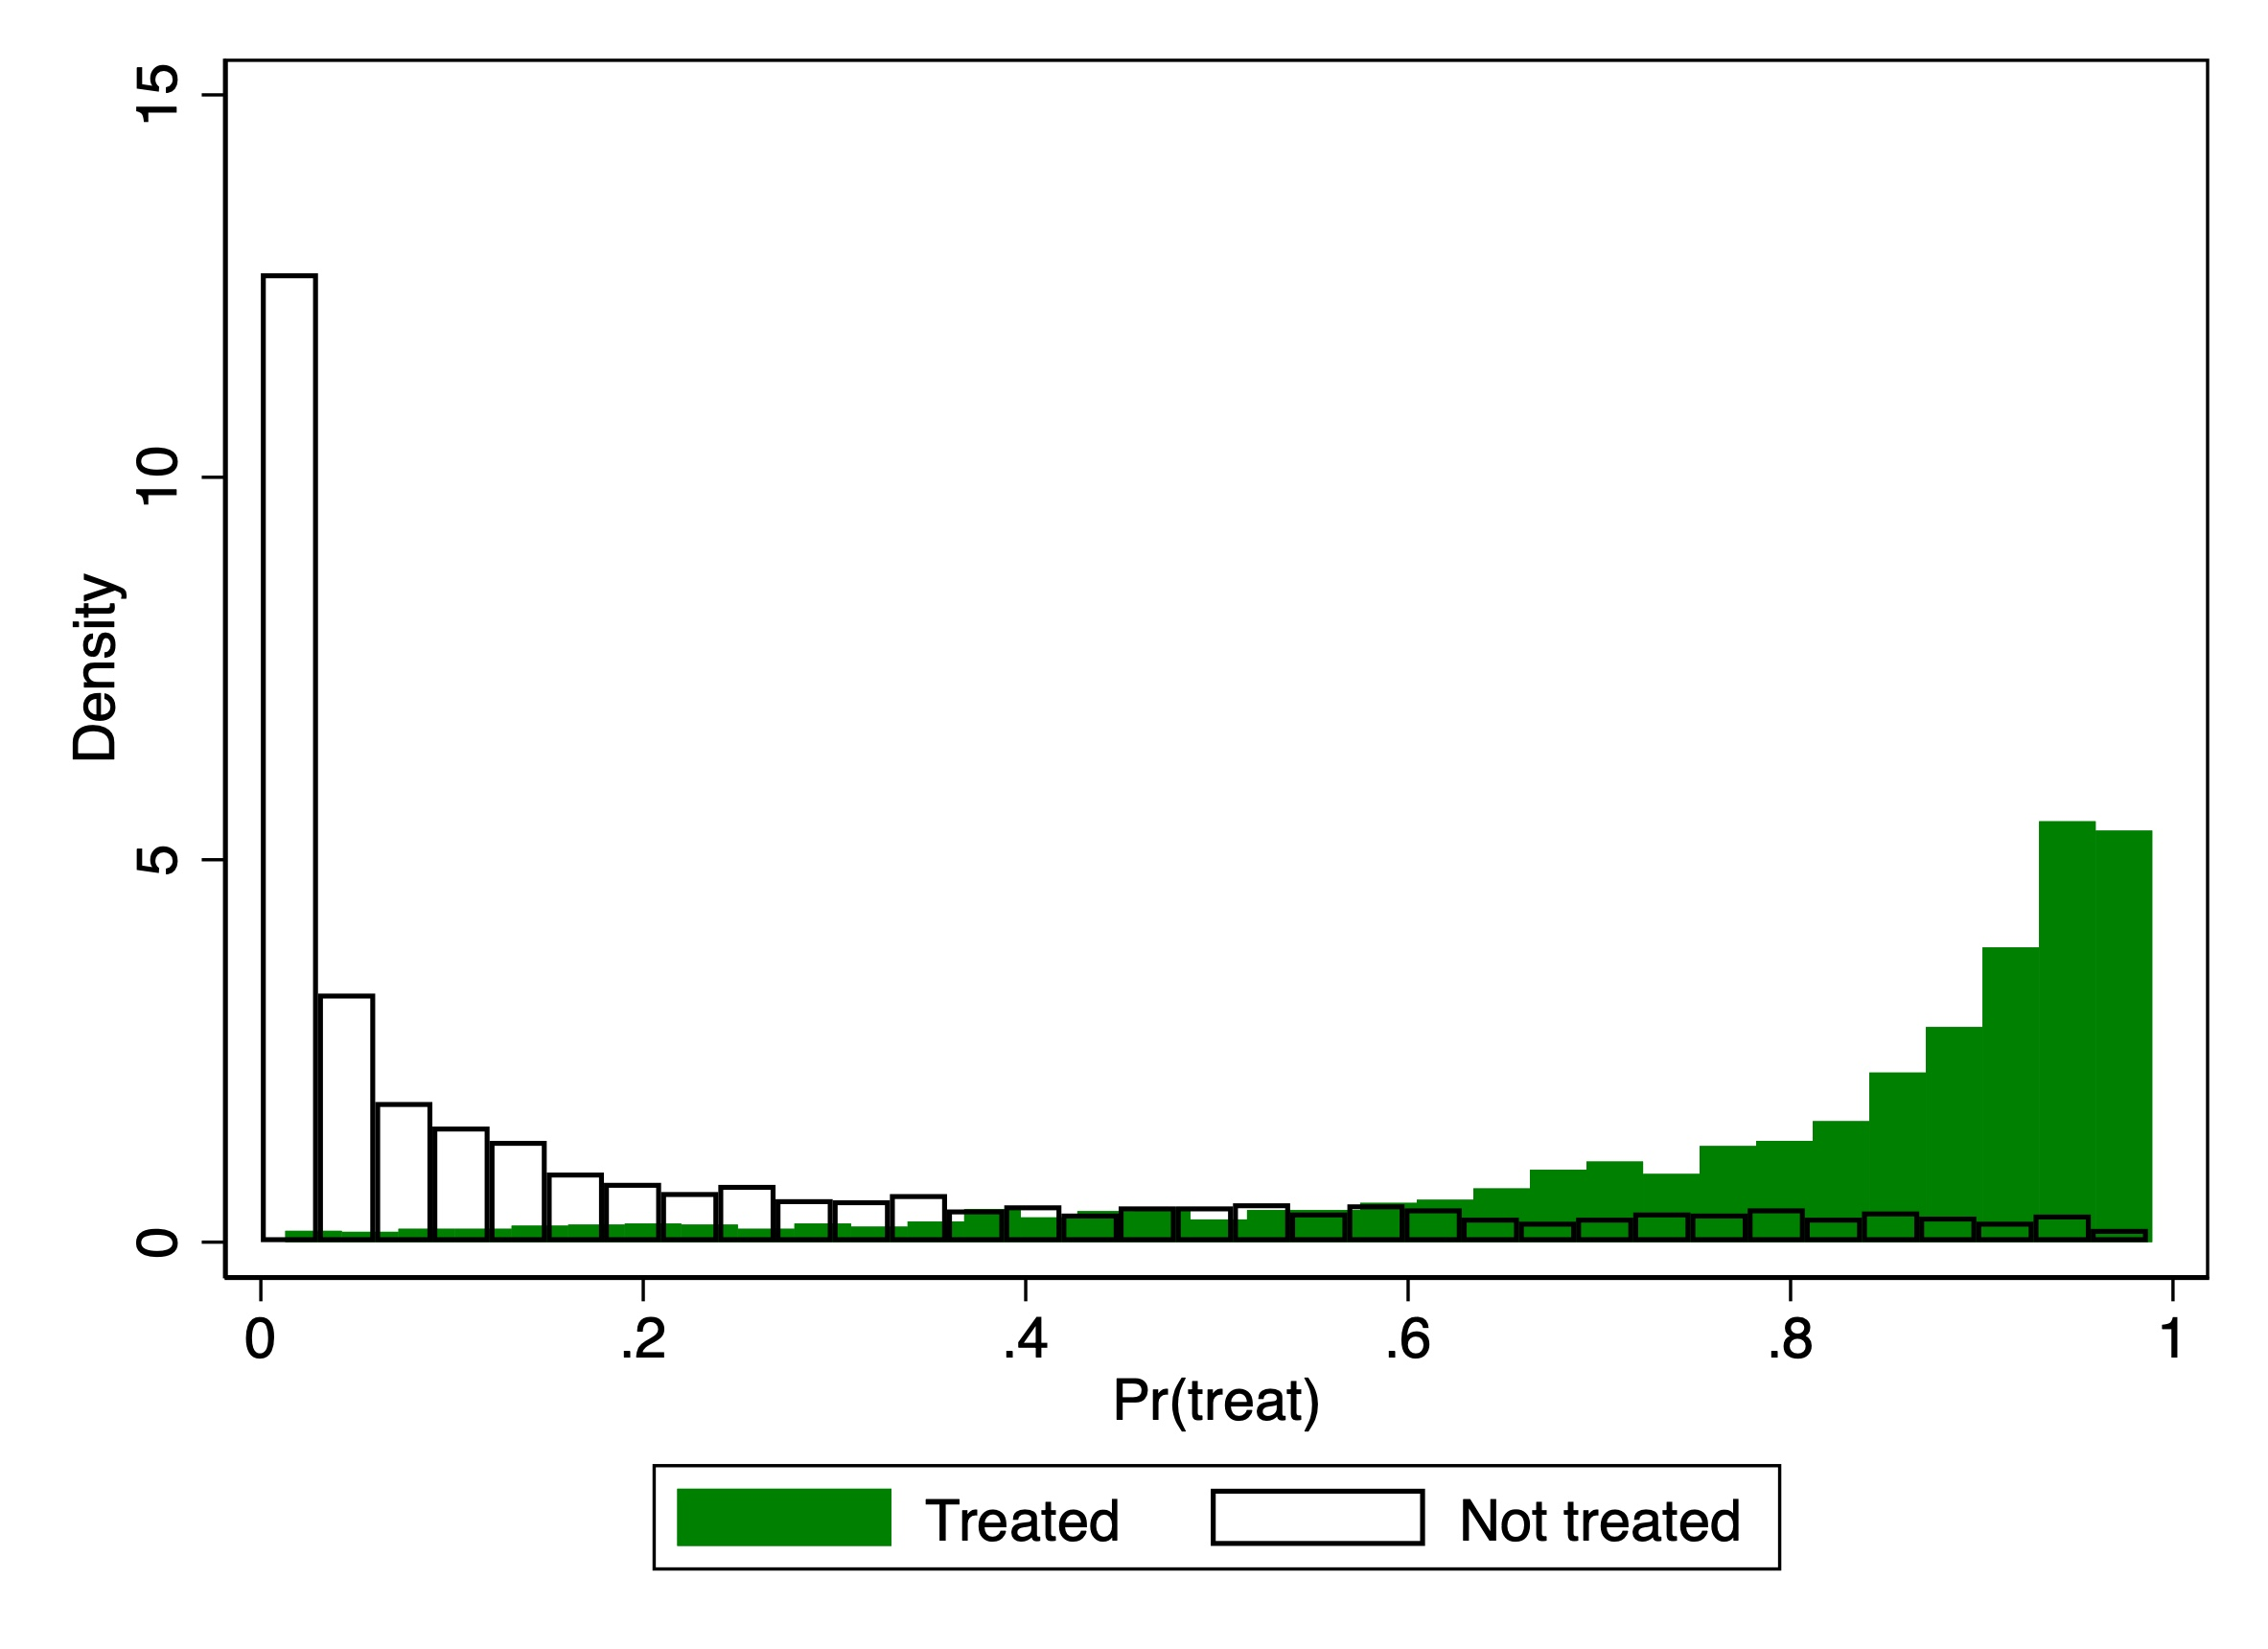
\includegraphics[scale=0.1]{./lecture_includes/covariate_imbalance.jpg}
\end{center}
\end{figure}

\end{frame}





\begin{frame}{Regression specifications 1 and 2}

We will look at several different specifications.  These first two are standard ways of incorporating covariates. You enter them in linearly as controls. 

\begin{eqnarray}
\text{earnings} &=& \beta_0 + \beta_1 \text{treat} + \beta_2 \text{age} + \beta_3 \text{gpa} + \epsilon \\
\text{earnings} &=& \beta_0 + \beta_1 \text{treat} + \beta_2 \text{age} + \beta_3 \text{age\_sq} + \beta_4 \text{gpa} \nonumber \\
&&+ \beta_5 \text{gpa\_sq} + \beta_6 (\text{gpa} \times \text{age}) + \epsilon 
\end{eqnarray}

\bigskip

Interpretation focuses on $\widehat{\beta_1}$.  But what does it mean?  Look at top two.  Remember ATE is 2500.

\end{frame}

\begin{frame}{ATE estimates across different specifications}

\begin{figure}
\begin{center}
             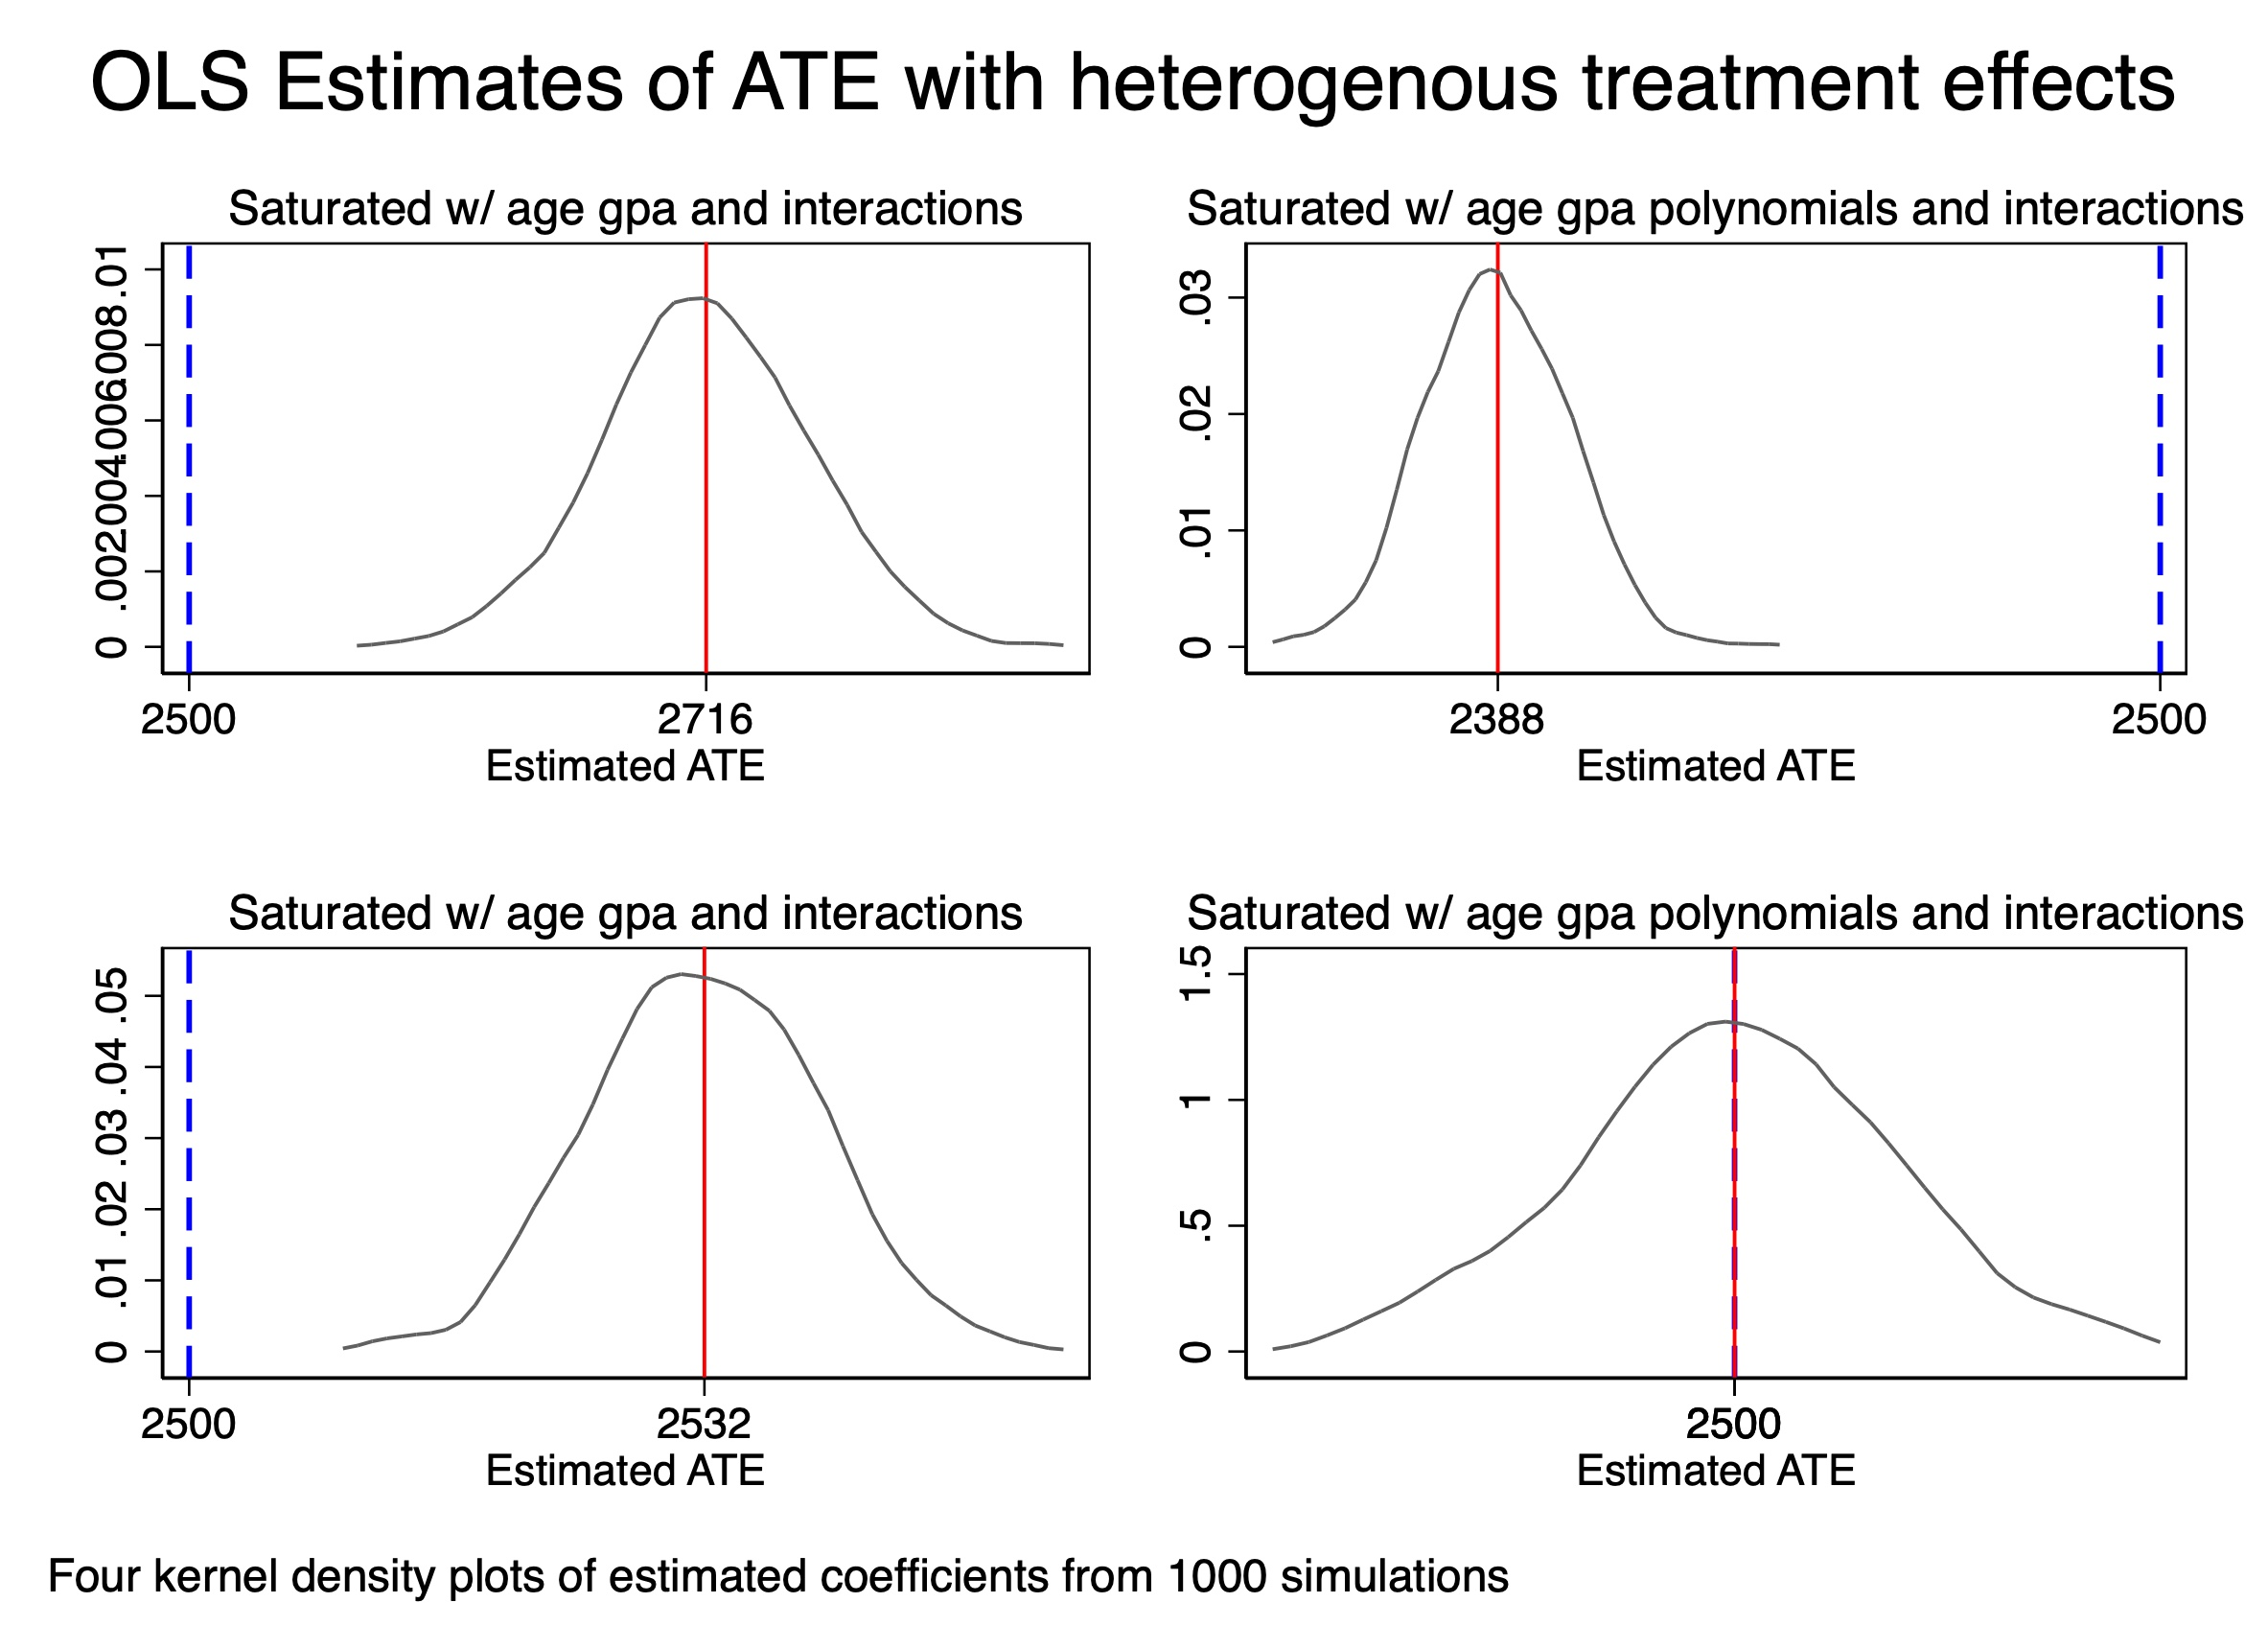
\includegraphics[scale=0.1]{./lecture_includes/combined_kernels_ate.jpg}
\end{center}
\end{figure}

\end{frame}


\begin{frame}{ATT Calculation: Regression 3}
\tiny

Saturated regressions: interact treatment dummy with all covariates. 

\begin{itemize}
\item Regression Specification:
\begin{eqnarray*}
\text{earnings} &=& \beta_0 + \beta_{1t} \text{treat} + \beta_{2a} \text{age} + \beta_{3g} \text{gpa} + \beta_{4ta} (\text{treat} \times \text{age}) + \beta_{5tg} (\text{treat} \times \text{gpa}) + \beta_{6age} (\text{age} \times \text{gpa})  \nonumber \\
&&+ \beta_{6tag} (\text{treat} \times \text{age} \times \text{gpa}) + \epsilon
\end{eqnarray*}

\bigskip

Estimated ATE is the coefficient, $\widehat{\beta_{1t}}$, but how do we get the estimated ATT?

\item Calculating ATT:
\begin{equation*}
    \text{ATT}_3 = \beta_{1t} + \beta_{4ta} \cdot \bar{\text{age}} + \beta_{5tg} \cdot \bar{\text{gpa}} + \beta_{6tag} \cdot \bar{\text{age}} \cdot \bar{\text{gpa}}
\end{equation*}using the means of all covariates

\end{itemize}
\end{frame}

\begin{frame}{ATT Calculation: Regression 4}


\tiny 
Saturated regressions: interact it with covariates, higher order polynomials, and all interactions


\begin{itemize}
\item Regression Specification:
\begin{eqnarray*}
\text{earnings} &=& \beta_0 + \beta_{1t} \text{treat} + \beta_{2a} \text{age} + \beta_{3a_sq} \text{age_sq} + \beta_{4g} \text{gpa} + \beta_{5g_sq} \text{gpa_sq} + \\
&& \beta_{6ta} (\text{treat} \times \text{age}) + \beta_{7ta_sq} (\text{treat} \times \text{age_sq}) + \beta_{8tg} (\text{treat} \times \text{gpa}) + \\
&& \beta_{9tg_sq} (\text{treat} \times \text{gpa_sq}) + \beta_{10ag} (\text{age} \times \text{gpa}) + \beta_{11a_sqg} (\text{age_sq} \times \text{gpa}) + \\
&& \beta_{12ag_sq} (\text{age} \times \text{gpa_sq}) + \beta_{13a_sqg_sq} (\text{age_sq} \times \text{gpa_sq}) + \epsilon
\end{eqnarray*}

\bigskip

Estimated ATE is the coefficient, $\widehat{\beta_{1t}}$, but how do we get the estimated ATT?

\item Calculating ATT:
\begin{eqnarray*}
\text{earnings} &=& \beta_0 + \beta_{1t} \text{treat} + \beta_{2a} \text{age} + \beta_{3a\_sq} \text{age\_sq} + \beta_{4g} \text{gpa} + \beta_{5g\_sq} \text{gpa\_sq} + \beta_{6ta} (\text{treat} \times \text{age})  \nonumber \\ 
&&+ \beta_{7ta\_sq} (\text{treat} \times \text{age\_sq}) + \beta_{8tg} (\text{treat} \times \text{gpa}) + \beta_{9tg\_sq} (\text{treat} \times \text{gpa\_sq}) + \beta_{10ag} (\text{age} \times \text{gpa})  \nonumber \\
&&+ \beta_{11a\_sqg} (\text{age\_sq} \times \text{gpa}) + \beta_{12ag\_sq} (\text{age} \times \text{gpa\_sq}) + \beta_{13a\_sqg\_sq} (\text{age\_sq} \times \text{gpa\_sq}) + \epsilon
\end{eqnarray*}
\end{itemize}
\end{frame}

\begin{frame}{Interpretations}

\begin{itemize}
\item ATE is 2500
\item ATT is 1980
\item Key point here: the same regression contains both parameters, but only when done correctly, and only when interpreted correctly
\end{itemize}

\end{frame}




\begin{frame}{ATE estimates across different specifications}

\begin{figure}
\begin{center}
             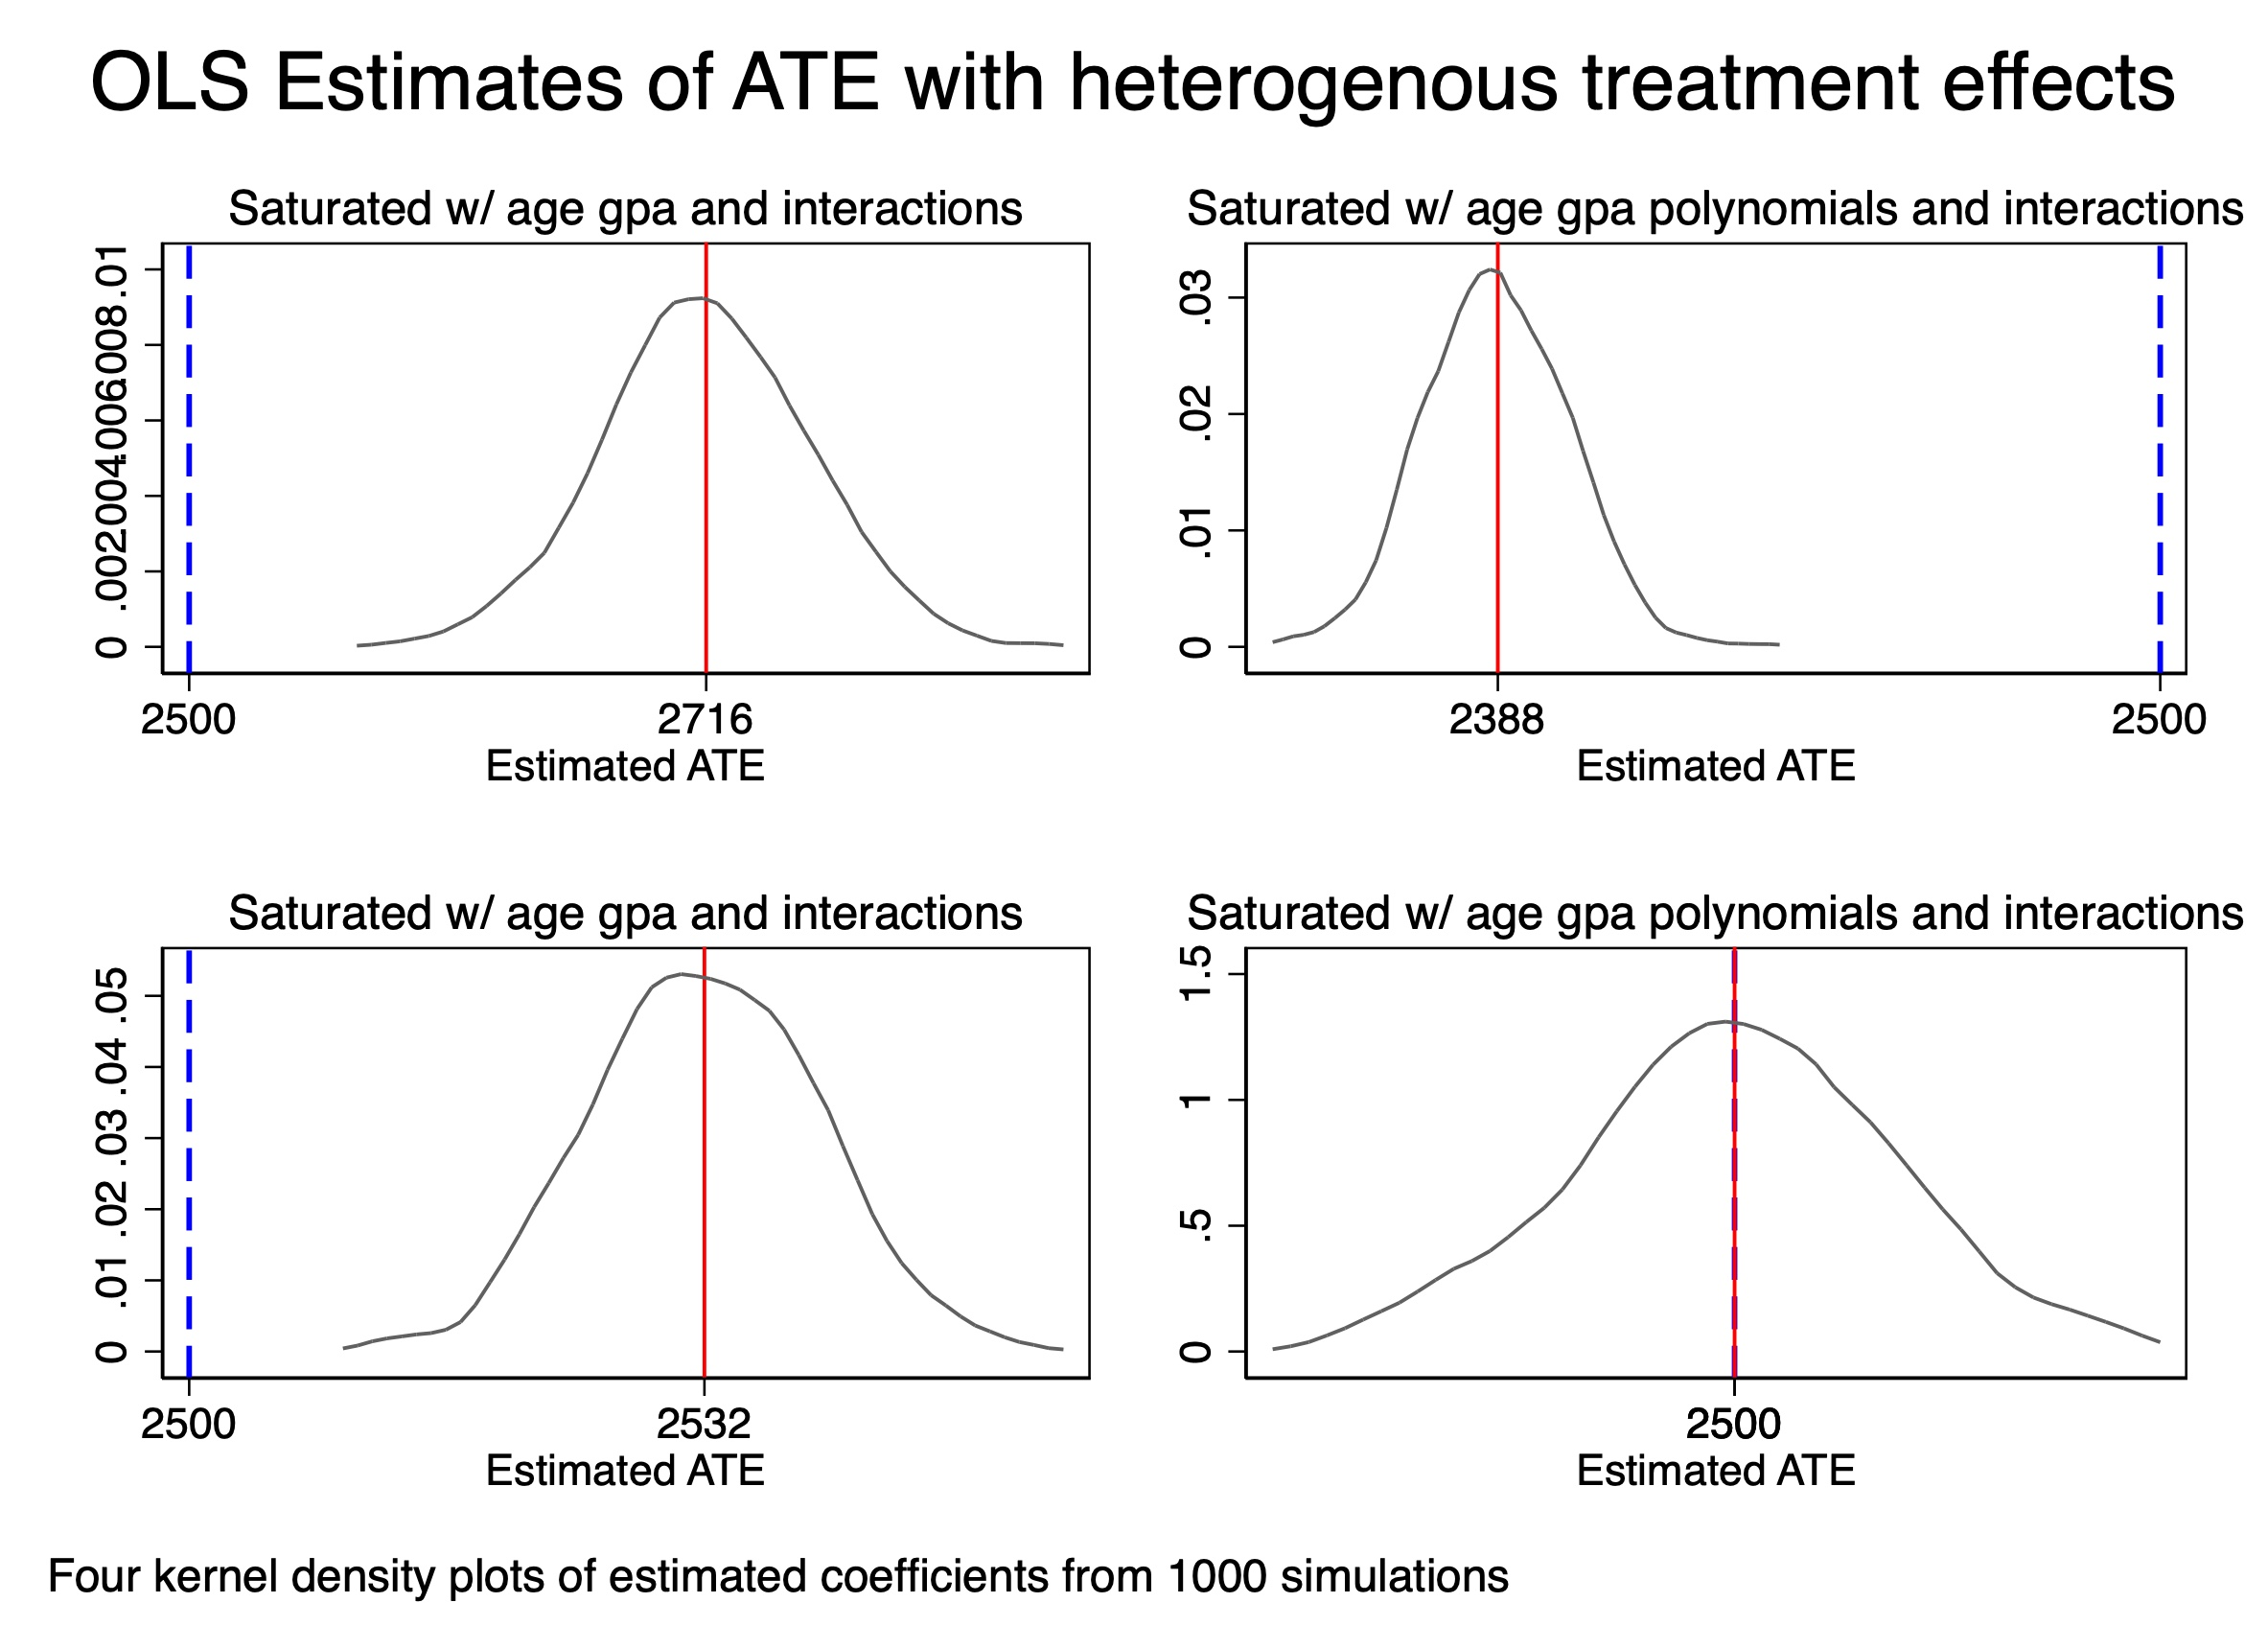
\includegraphics[scale=0.1]{./lecture_includes/combined_kernels_ate.jpg}
\end{center}
\end{figure}

\end{frame}



\begin{frame}{ATT estimates across different specifications}

\begin{figure}
\begin{center}
             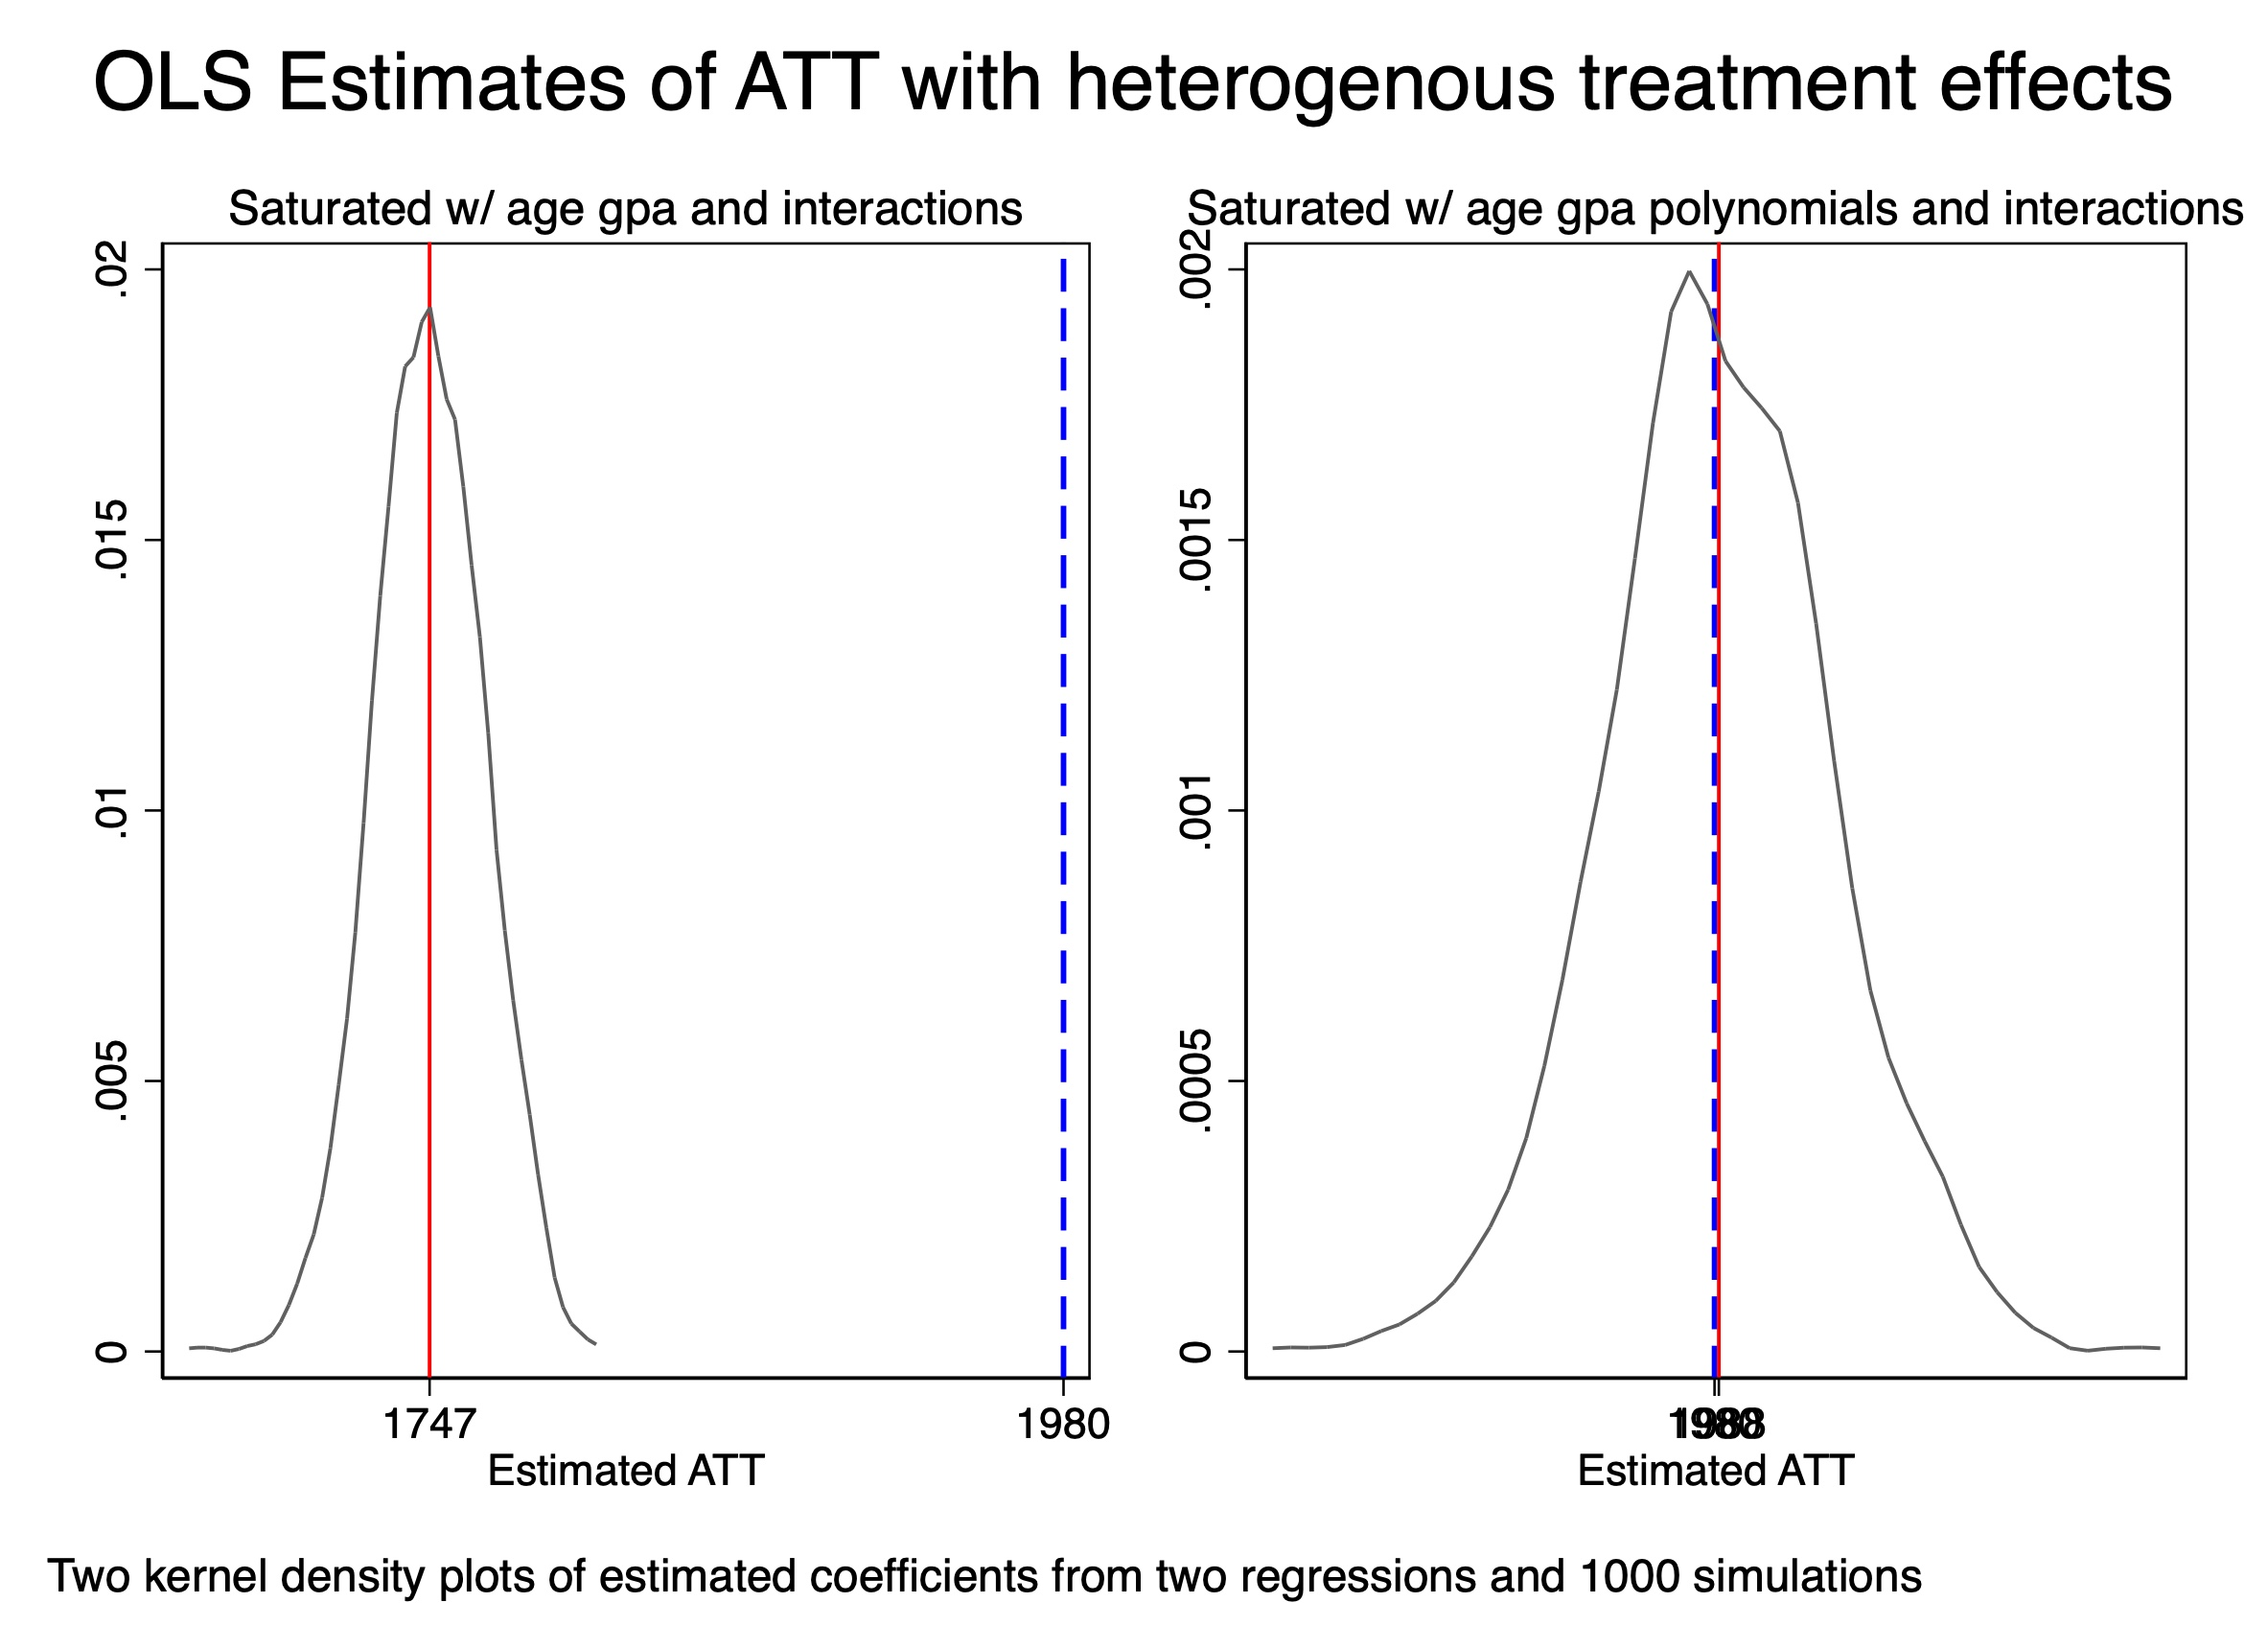
\includegraphics[scale=0.1]{./lecture_includes/combined_kernels_att.jpg}
\end{center}
\end{figure}

\end{frame}


\begin{frame}{Matching by minimizing Maha distance metric}

\begin{itemize}
\item Next I just estimated the ATT using a simpler model -- nonparametric matching using Abadie and Imbens (2006;2011)
\item It's biased when the matches aren't exact, but you can use regression adjustment to estimate the selection bias
\item Similar to what augmented synth does 
\item Much less difficult syntax
\end{itemize}

\end{frame}

\begin{frame}{ATT estimates across different matching specifications}

\begin{figure}
\begin{center}
             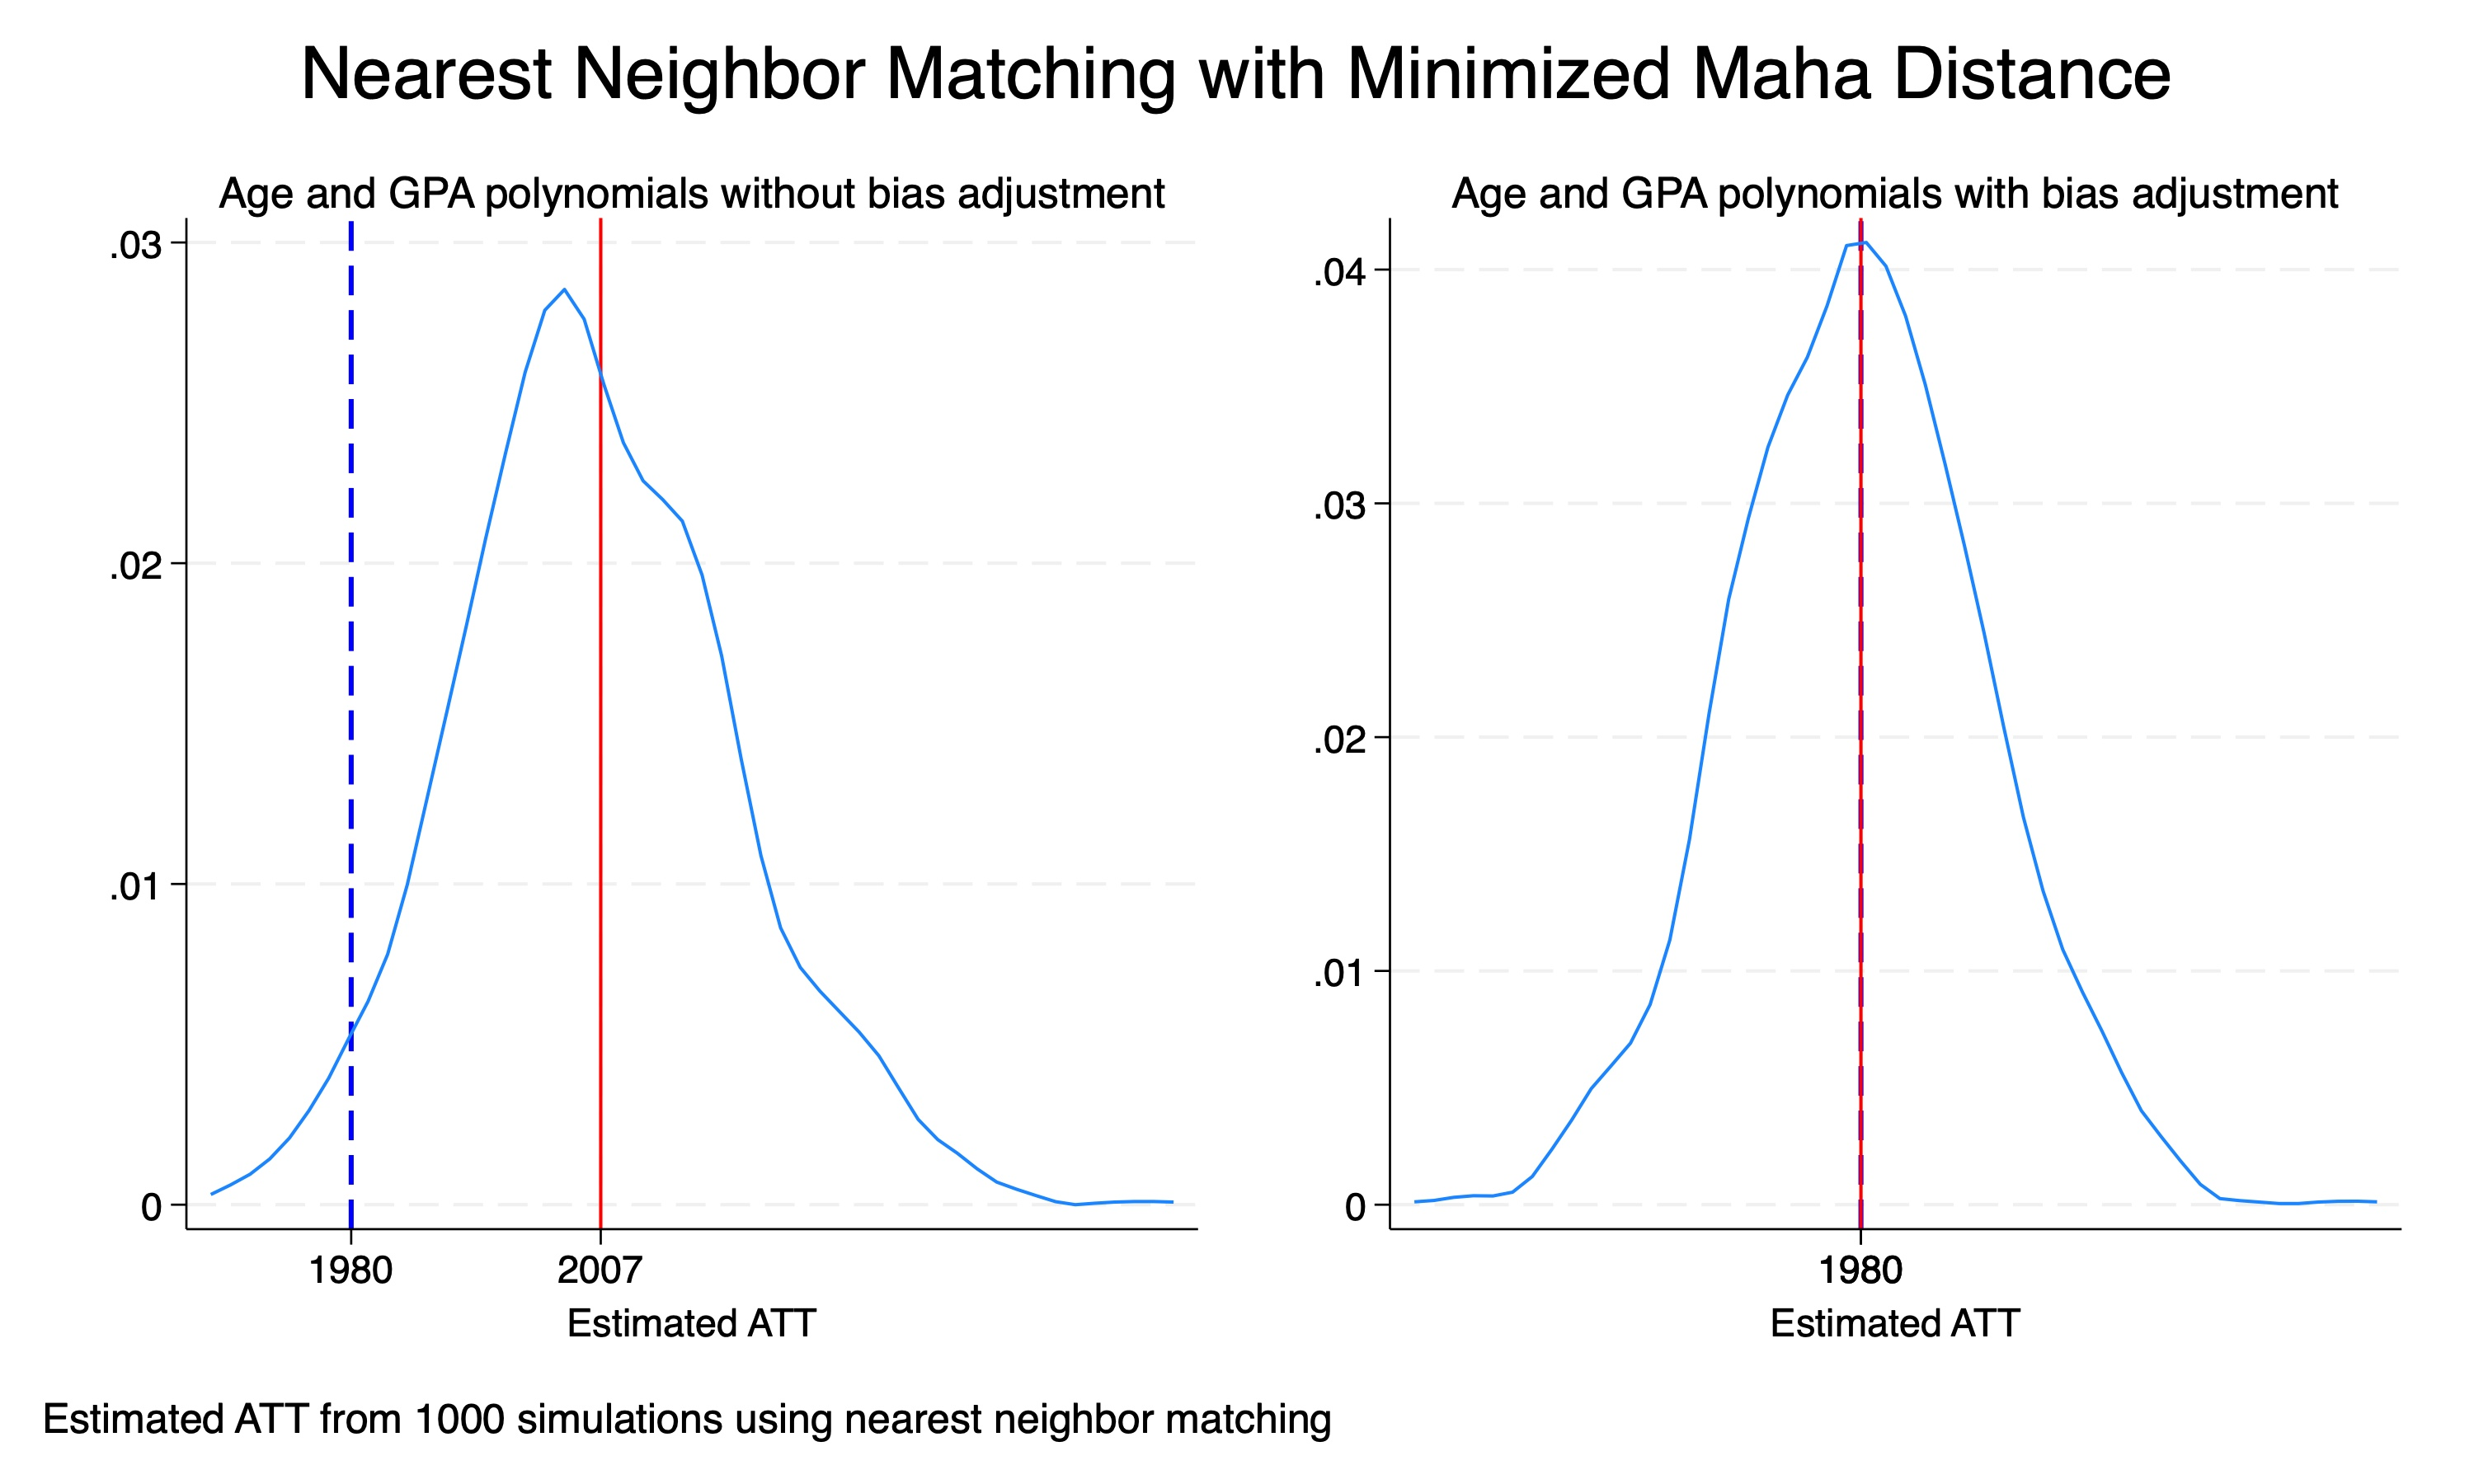
\includegraphics[scale=0.1]{./lecture_includes/combined_kernels_maha.jpg}
\end{center}
\end{figure}

\end{frame}


\begin{frame}{Recommended steps of causal projects}

\begin{enumerate}
\item Define the parameter we want (``ATT''), 
\item Ask what what beliefs do you need (``identification''), and 
\item Build cranks that produce the correct numbers (``estimator'')
\end{enumerate}

\bigskip

See how when we skep 1 and 2 and go straight to 3, heterogenous treatment effects makes major problems for interpretation?  It isn't that regressions can't recover parameters, but you have to saturate when you're attempting to recover ATE or ATT, and even then it's challenging to interpret -- and programming, you often don't have code that will do it for you.

\end{frame}



\subsection{Average causal response functions}


\begin{frame}{Introducing a new causal parameter}



\begin{itemize}
\item \textbf{ATT}: Extensive margin causal parameter.  Do this versus don't do this.
\item \textbf{Dose}: Intensive margin causal parameter.  Do this much versus this much.
\end{itemize}

\bigskip

The dose causal parameter will be based on Angrist and Imbens (1995)

\end{frame}




\begin{frame}{Parameters}

\begin{block}{Average treated on the treated}
$ATT(d|d) = E[Y^d_{it} - Y^0_{it} | D_{it}=d]$
\end{block}

\bigskip

while the treatment, $D$, can be any amount, $d$, that amount is technically a particular dose.  We raised the minimum wage, but we raised it to a particular wage. 

\end{frame}


\begin{frame}{Parameters}

\begin{block}{Average treated on the treated}
$ATT(d|d) = E[Y^d_{it} - Y^0_{it} | D_{it}=d]$
\end{block}

\bigskip

This is ``the ATT of $d$ for the groups that chose $d$ dosage'' which uses as its comparison no dose.

\end{frame}

\begin{frame}{Average causal response function}

\begin{figure}
\begin{center}
             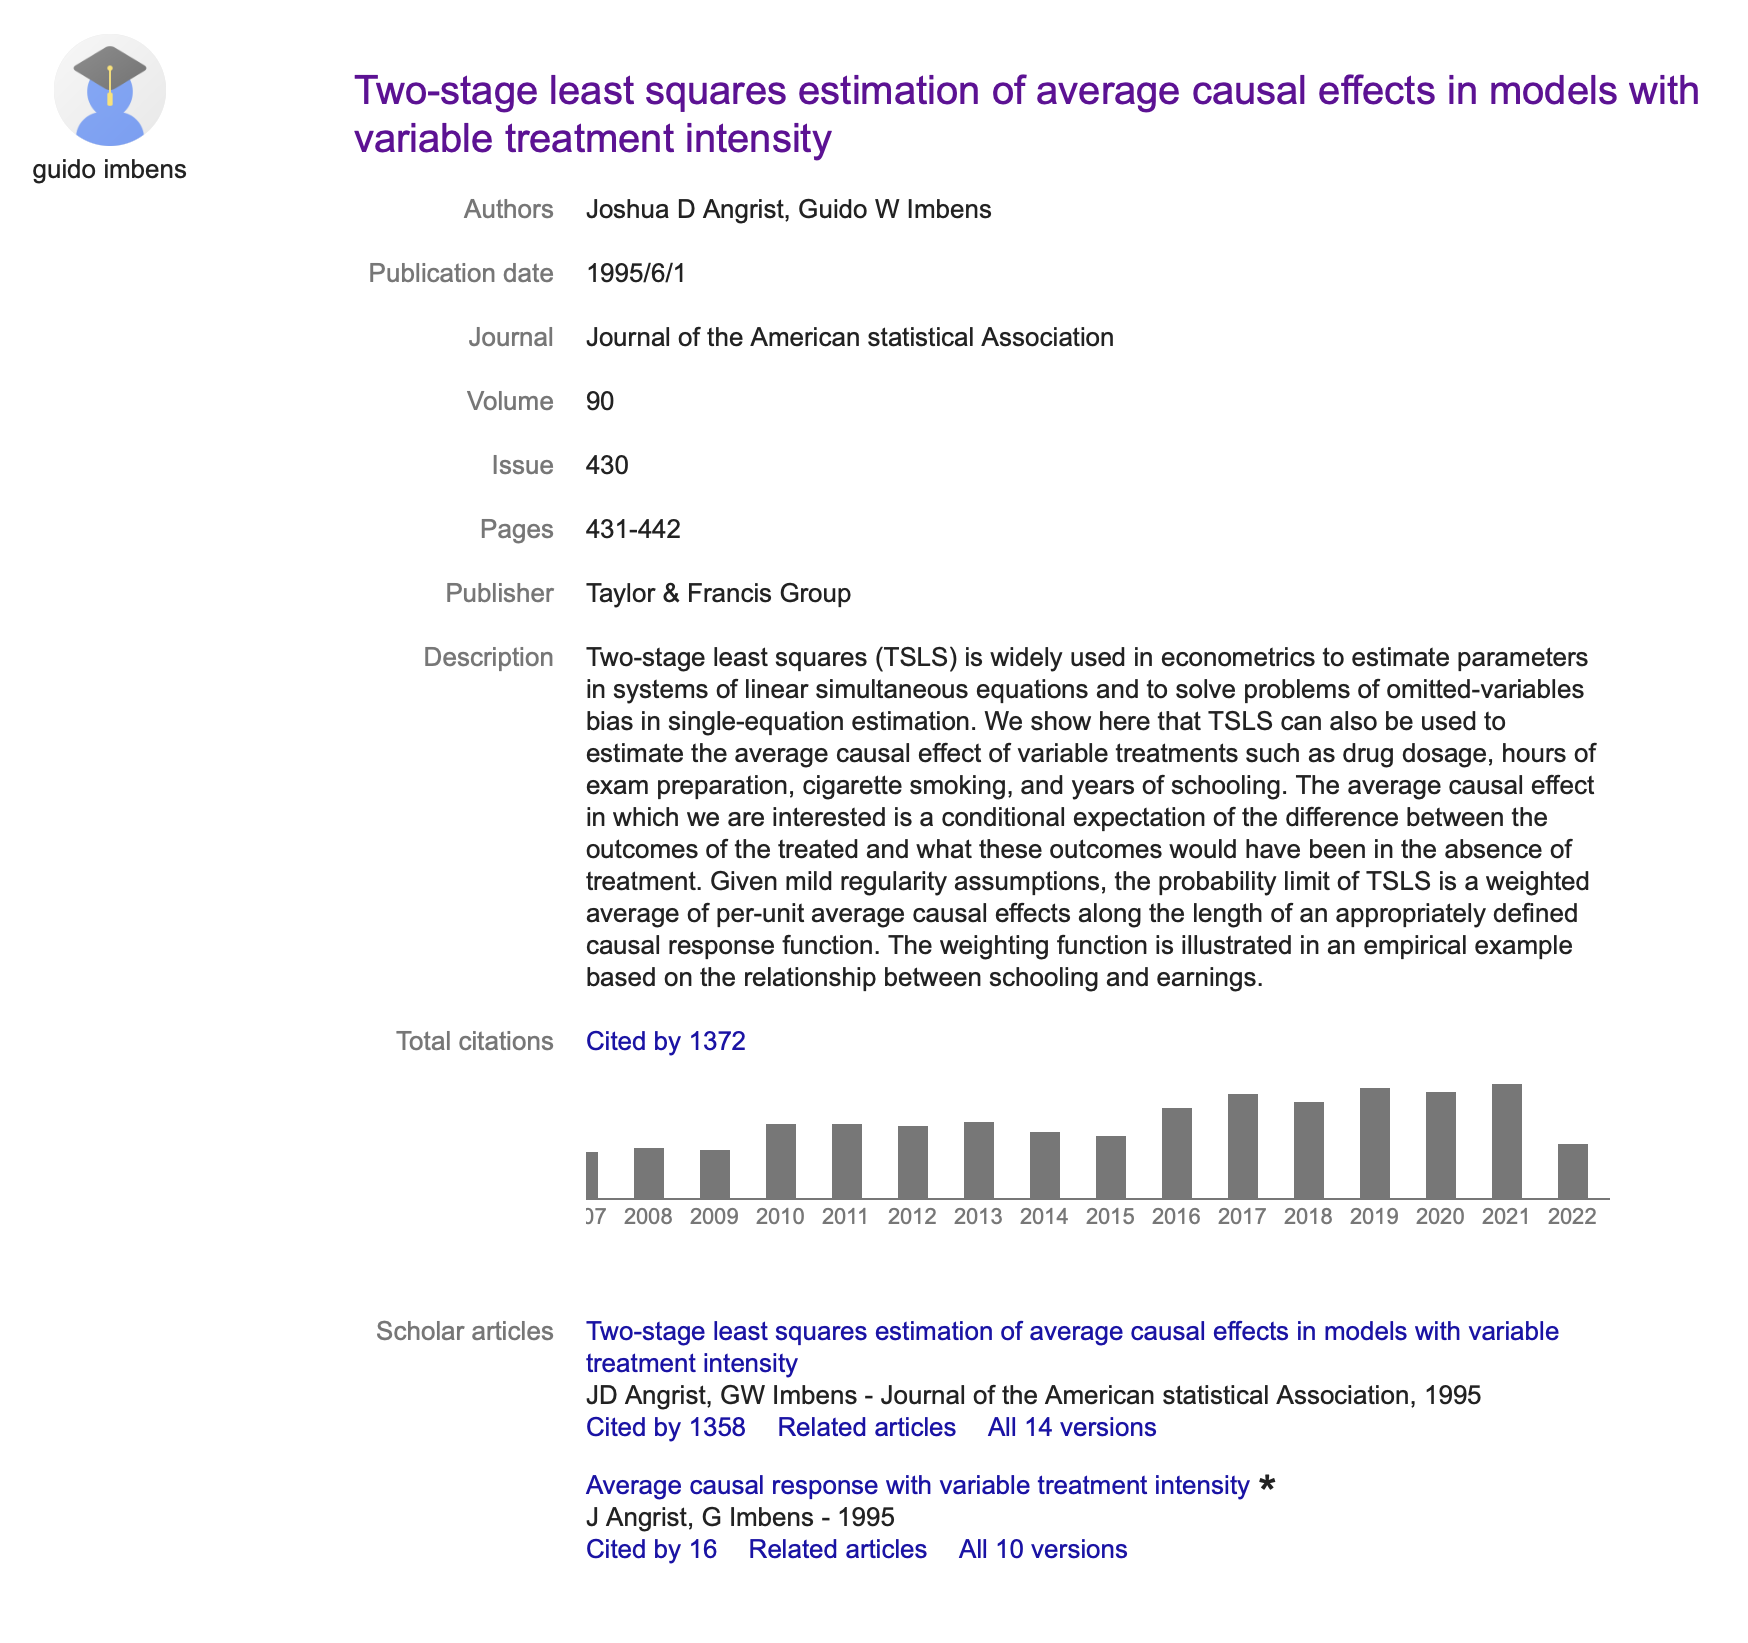
\includegraphics[scale=0.3]{./lecture_includes/angrist_imbens_IV_intensity}
\end{center}
\end{figure}

\end{frame}


\begin{frame}{Angrist and Imbens 1995}

\begin{quote}
``We refer to the parameter $\beta$ as the \textbf{average causal response (ACR)}. This parameter captures a weighed average causal responses to a unit change in treatment, for those whose treatment status is affected by the instrument. \dots ''
\end{quote}

\end{frame}


\begin{frame}{ATT for a given dose}

\begin{figure}
\begin{center}
             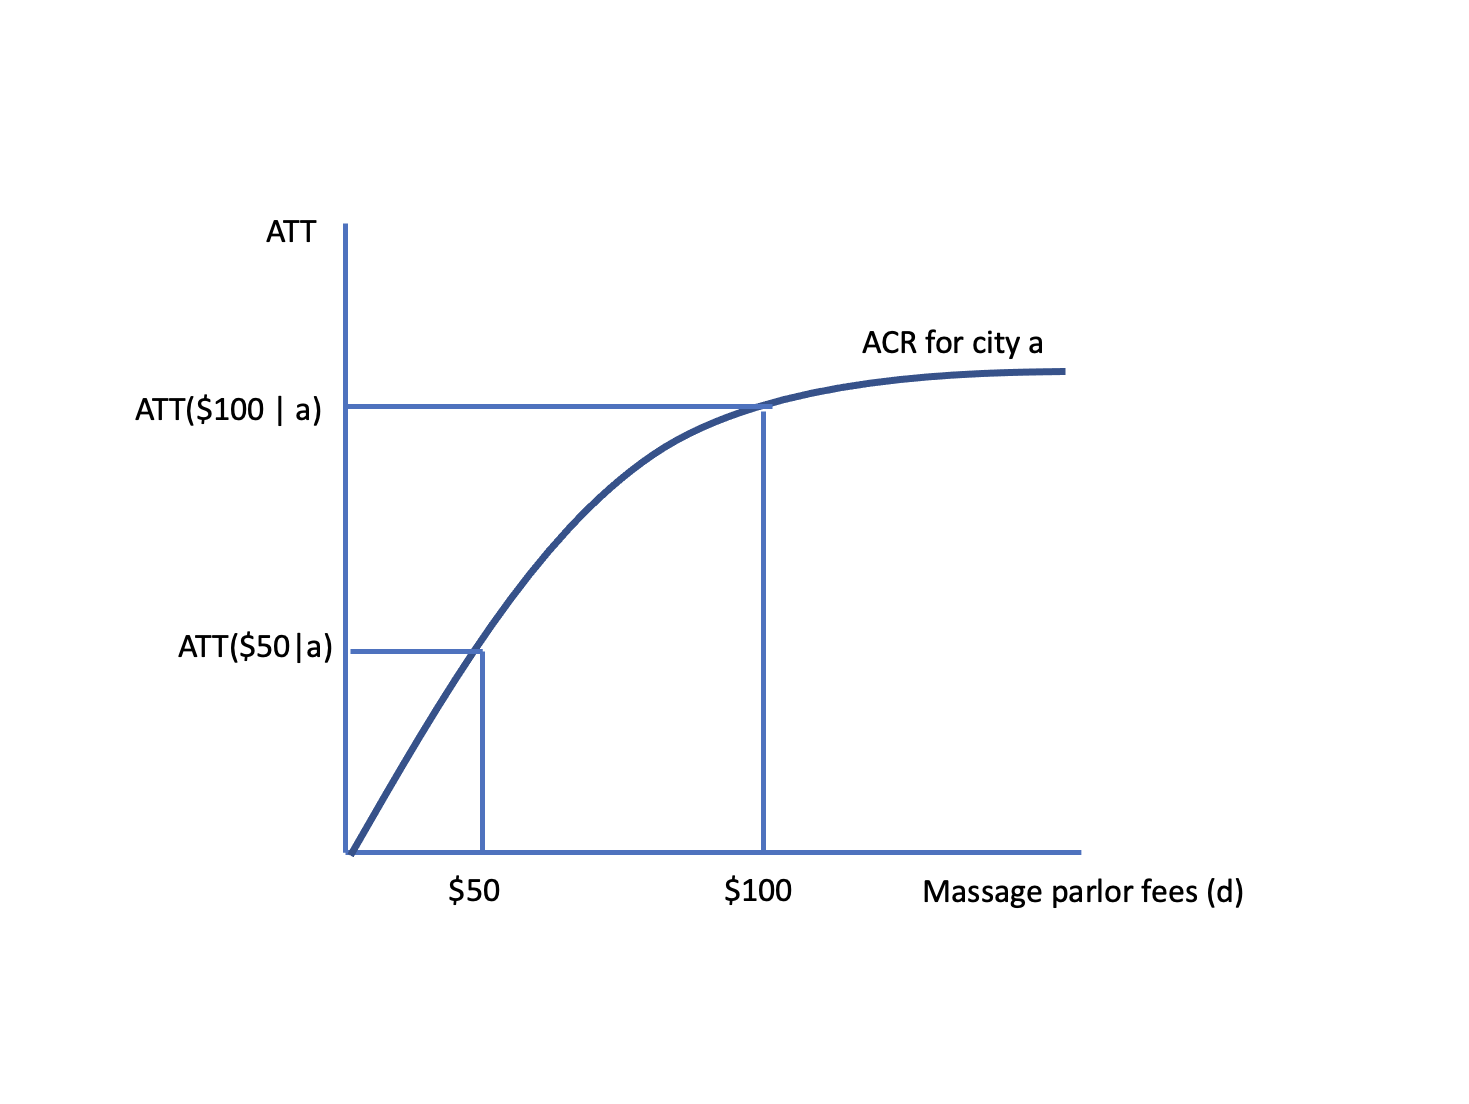
\includegraphics[scale=0.3]{./lecture_includes/acrt_fig1.png}
\end{center}
\end{figure}

What is the effect of setting fees to \$100 versus nothing at all? It's ATT(\$100$|$a) for this city.


\end{frame}

\begin{frame}{ATT for a given dose}

\begin{figure}
\begin{center}
             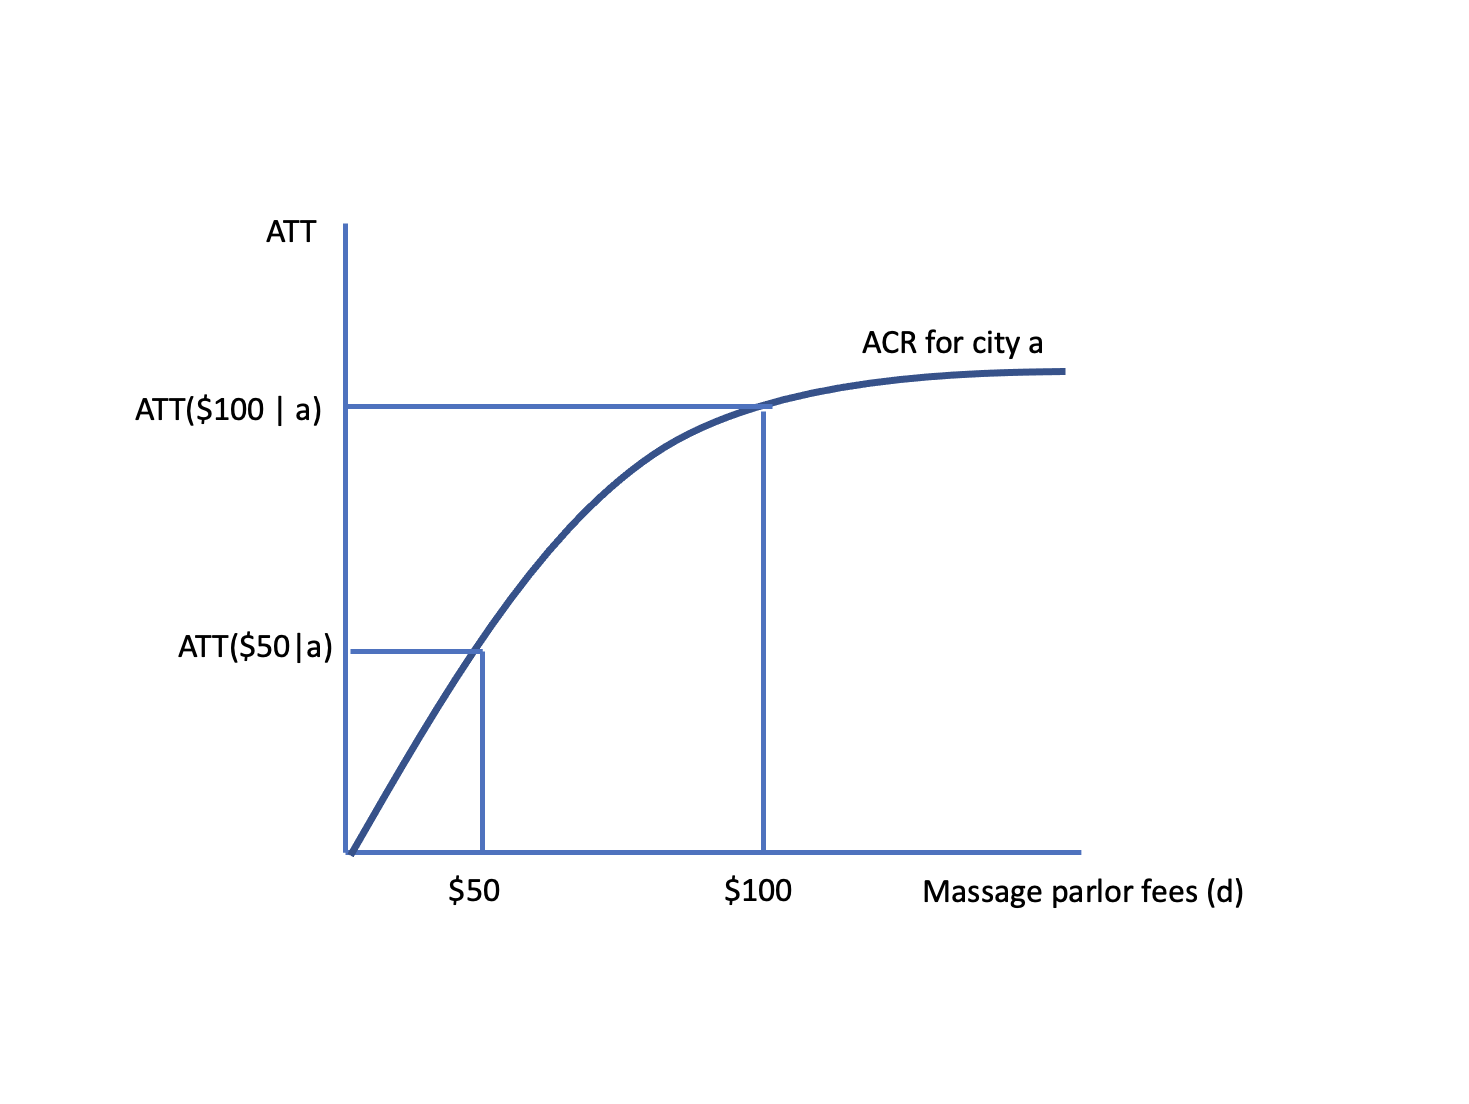
\includegraphics[scale=0.3]{./lecture_includes/acrt_fig1.png}
\end{center}
\end{figure}

Assume city $a$ did choose $d=\$100$. Then ATT(\$50$|$a) just means that that is its ATT \emph{had} it chosen the lower level.  The curve, in other words, is tracing out all average causal response for this city.


\end{frame}


\begin{frame}{ATT for a given dose}

\begin{figure}
\begin{center}
             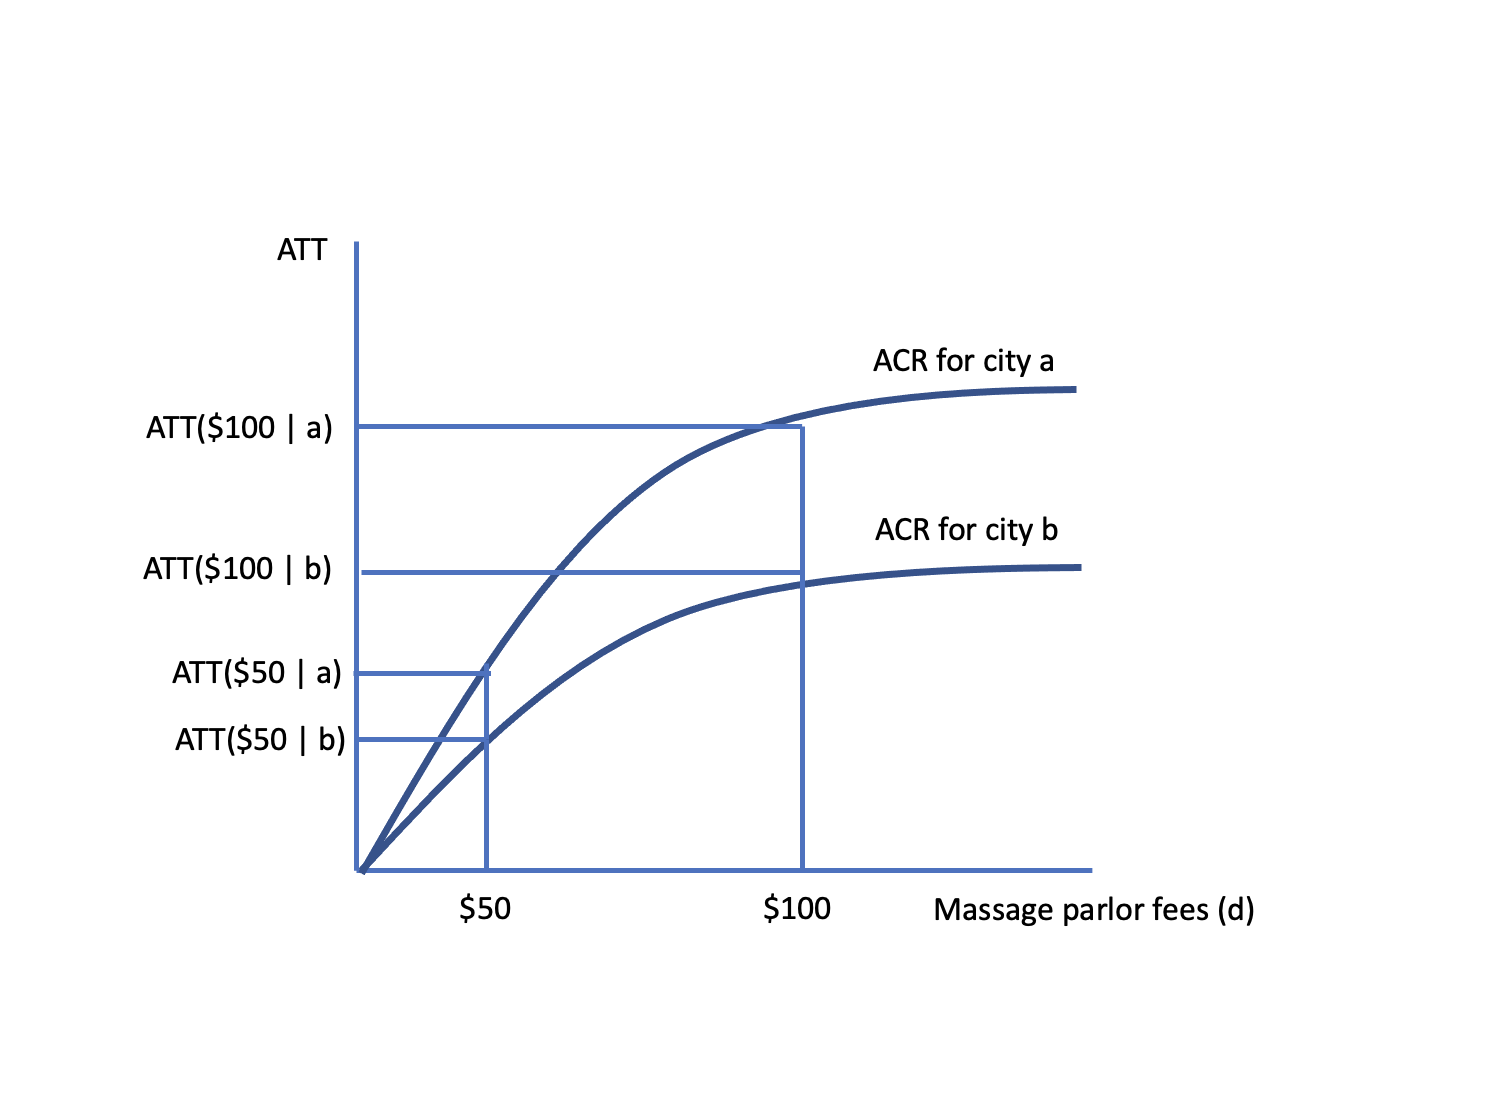
\includegraphics[scale=0.3]{./lecture_includes/acrt_fig2.png}
\end{center}
\end{figure}

What if everyone has different responses?  In other words, city $a$ has the higher curve than city $b$.  Then there are several comparisons possible.  What is the effect of \$50 on outcomes for cities that actually chose \$50 versus those than actually chose \$100?  

\end{frame}



\begin{frame}{Parameters}

\begin{block}{Average treated on the treated}
$ATT(d|d) = E[Y^d_{it} - Y^0_{it} | D_{it}=d]$
\end{block}

\bigskip

Notice that you are comparing any dose $d$ to no treatment at all -- sort of an extensive margin causal response, but that isn't the only causal concept we have.  Elasticities are causal, demand curves are causal, but they aren't based on comparisons to nothing -- they are intensive margin comparisons, local comparisons, adjacencies. Zero isn't the only counterfactual in other words.

\end{frame}
\begin{frame}


\begin{figure}
\begin{center}
             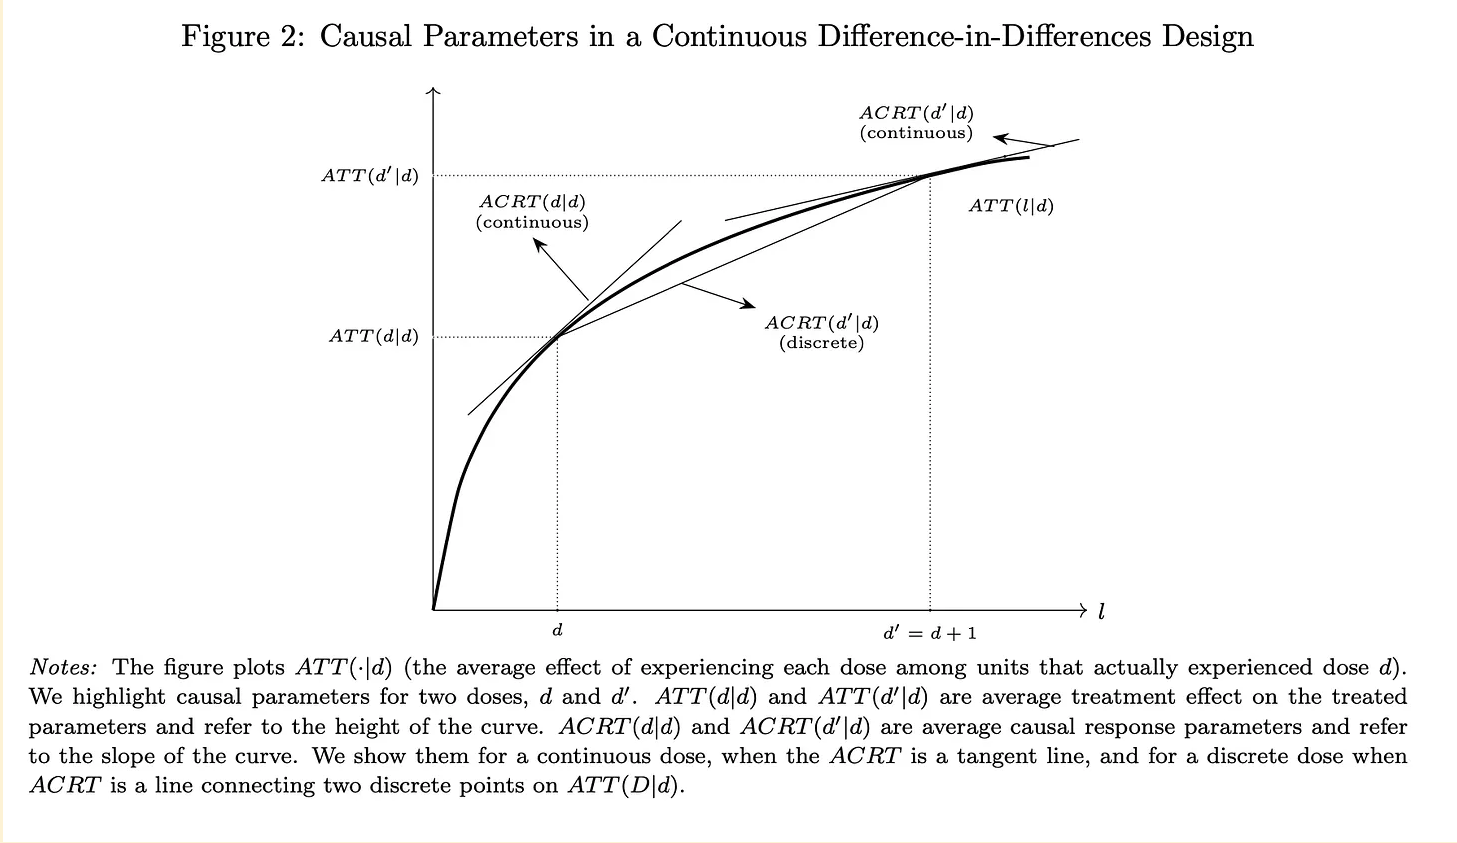
\includegraphics[scale=0.45]{./lecture_includes/continuous1.png}
\end{center}
\end{figure}

\end{frame}

\begin{frame}{What is the ACRT?}

\begin{itemize}
\item ACRT is the causal effect of dose $D=d_j$ vs a different dose $D=D_{j-1}$ for group $d$
	\begin{itemize}
	\item Easiest example is the demand function: at $p=\$10$, I buy 10 units, but at $p=\$11$, I buy 5 units.  
	\item Causal effect of that one dollar increase is $-5$ units
	\item Demand curves are pairs of potential outcomes and treatments and equilibrium ``selects'' one of them
	\end{itemize}
\item Discrete/multi-valued treatment is linear difference between two ATTs for the same city
\item Continuous treatment is the derivative of the function itself
\end{itemize}

\end{frame}

\begin{frame}{Definition of the ACRT}

\begin{figure}
\begin{center}
             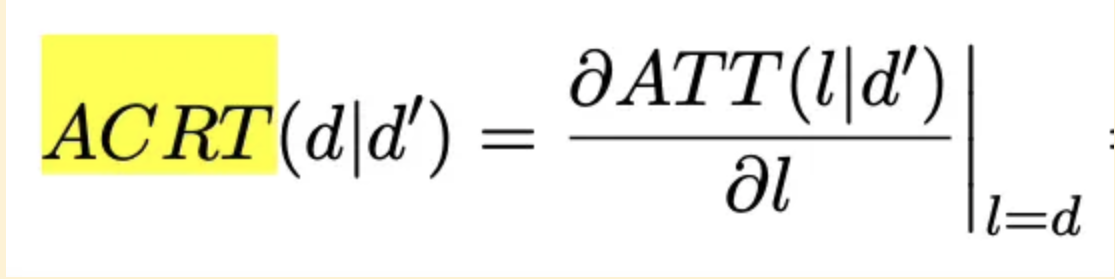
\includegraphics[scale=0.3]{./lecture_includes/continuous4.png}
\end{center}
\end{figure}

\end{frame}



\begin{frame}{Derivation of ACRT}

\begin{figure}
\begin{center}
             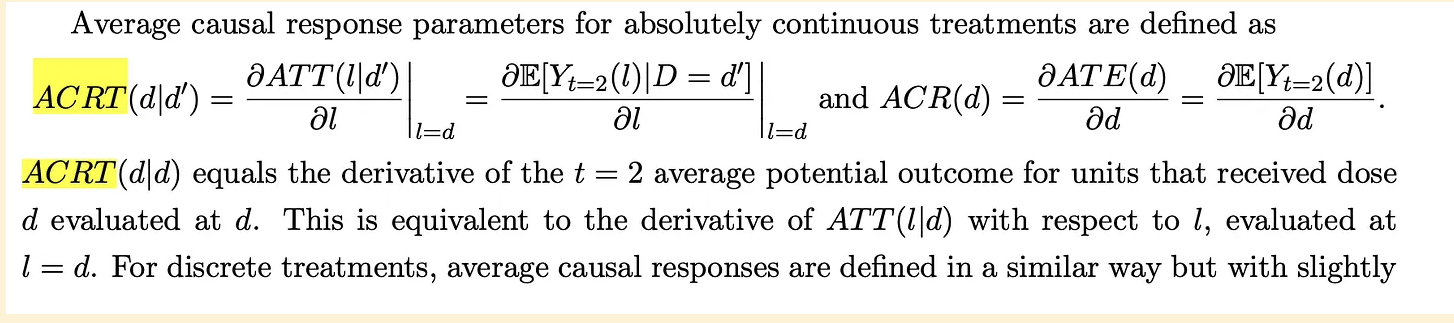
\includegraphics[scale=0.45]{./lecture_includes/continuous2.png}
\end{center}
\end{figure}

\end{frame}
\begin{frame}{Heterogeneities}


\begin{figure}{}
\begin{center}
             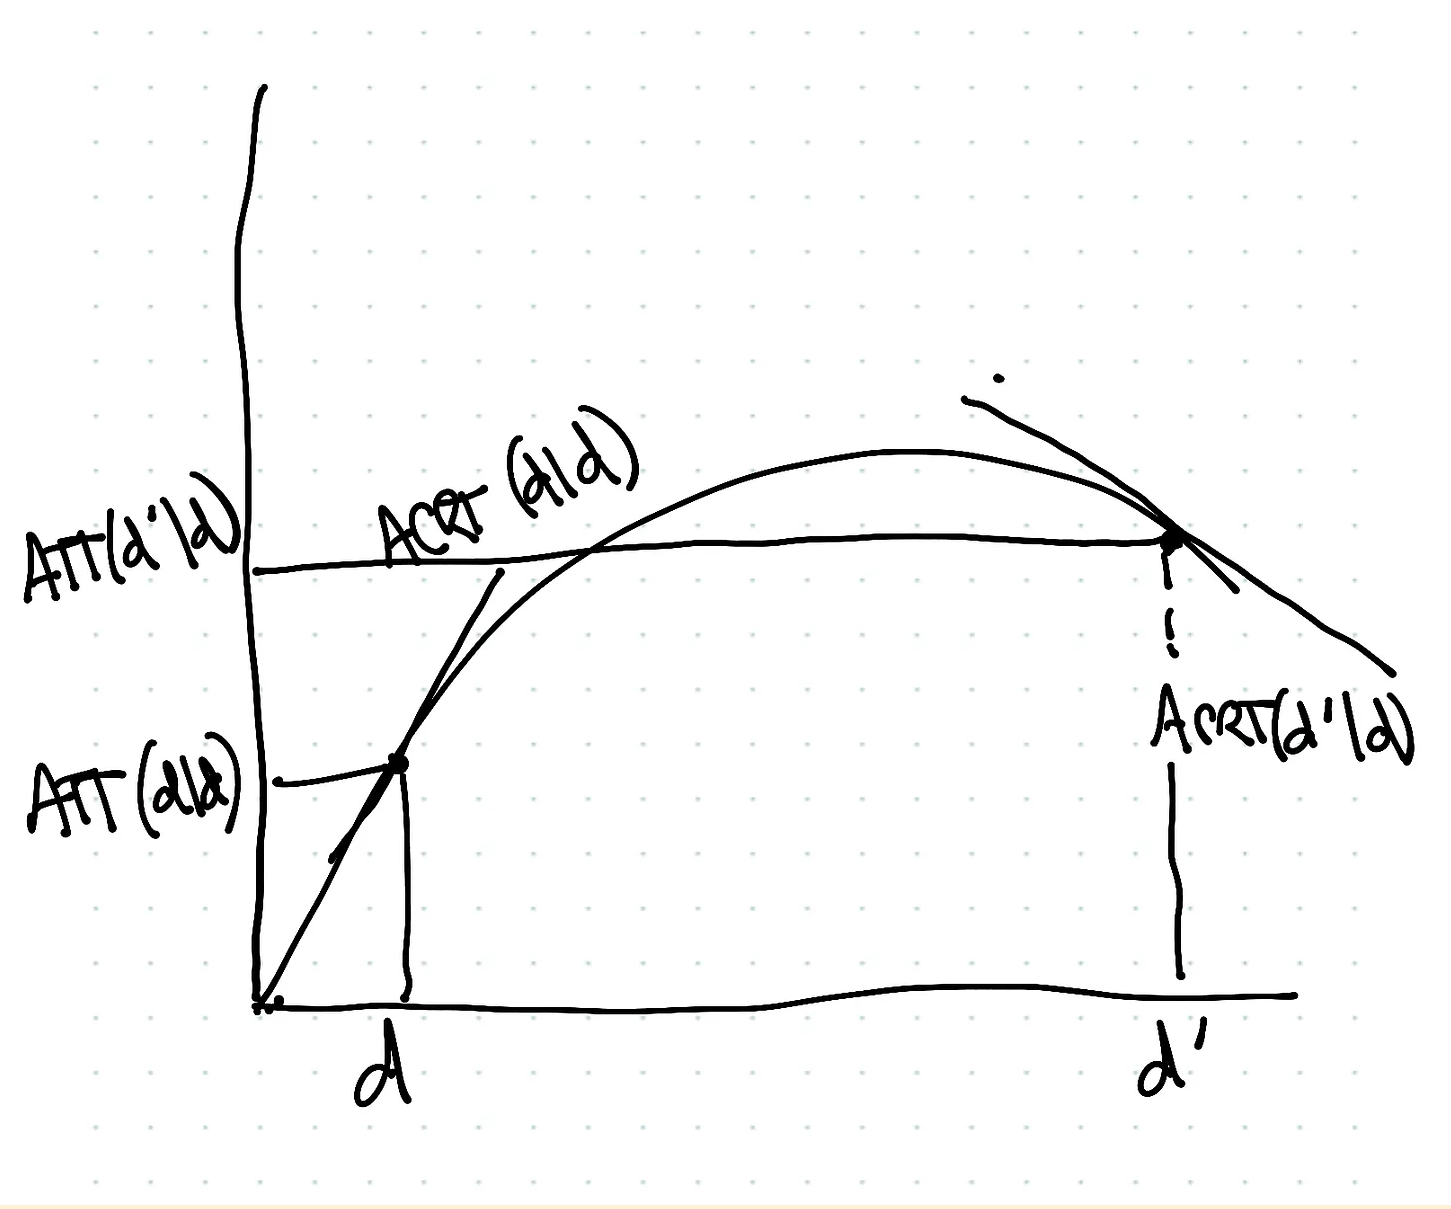
\includegraphics[scale=0.4]{./lecture_includes/continuous3.png}
\end{center}
\end{figure}

\end{frame}








\subsection{Identification}

\begin{frame}{Assumptions}

The authors lay out 5 assumptions, but I’m going to focus on 4. They are:

\begin{enumerate}
\item Random sampling
\item Continuous (2a) and Multi-Valued Treatment (2b)
\item No Anticipation and Observed Outcomes
\item Parallel trends
\end{enumerate}

\end{frame}

\begin{frame}{Identifying $ATT(d|d)$}

We can estimate the $ATT(d|d)$ using the simple DiD equation:

\begin{eqnarray*}
E [ \Delta Y_{it} | D_i = d] - E[ \Delta Y_{it} | D_i = 0]
\end{eqnarray*}

\bigskip

No anticipation and parallel trends converts this comparison of before and after into the $ATT(d|d)$

\bigskip

$ATT(d|d)$ is using as its counterfactual the ``no treatment'', note.  Treatment is a dosage compared to zero iow.

\end{frame}


\begin{frame}{Identifying ACRT}


\begin{eqnarray*}
ATT(b|b) - ATT(a|a) &=& ( E[ \Delta Y_{it} | D_i =a ] - E[ \Delta Y_{it} | D_i = 0]) \\
&& - ( E[ \Delta Y_{it} | D_i =b ] - E[ \Delta Y_{it} | D_i = 0]) \\
&=& E [ \Delta Y_{it} | D_i=a] - E[\Delta Y_{it} | D_i=b]
\end{eqnarray*}

Comparing high and low dose groups.

\end{frame}

\begin{frame}{Identifying ACRT}


\begin{eqnarray*}
ATT(d_j|d_j) - ATT(d_{j-1} | d_{j-1}) &=& \\
( ATT(d_j|d_j) - ATT(d_{j-1} | d_{j}) ) + ( ATT(d_{j-1} | d_j) - ATT(d_{j-1} | d_{j-1}) )&=&  \\
 ( \textcolor{blue}{ACRT(d_j | d_j)} ) + ( \textcolor{red}{ATT(d_{j-1} | d_j) - ATT(d_{j-1} | d_{j-1})} )&=&  \\
\end{eqnarray*}

Part in blue is the movement along the average causal response function, the ACRT, and is causal.  The part in red is selection bias. 

\end{frame}

\begin{frame}{Identifying ACRT}


\begin{eqnarray*}
ATT(d_j|d_j) - ATT(d_{j-1} | d_{j-1}) &=& \\
( ATT(d_j|d_j) - ATT(d_{j-1} | d_{j}) ) + ( ATT(d_{j-1} | d_j) - ATT(d_{j-1} | d_{j-1}) )&=&  \\
 ( \textcolor{blue}{ACRT(d_j | d_j)} ) + ( \textcolor{red}{ATT(d_{j-1} | d_j) - ATT(d_{j-1} | d_{j-1})} )&=&  \\
\end{eqnarray*}

Notice parallel trends allows to identify ATT terms but we need additional assumptions for this red part to vanish. We must assume that the ATT for cities that chose $d_j$ and cities that chose $d_{j-1}$ are the same had they both chose $d_{j-1}$.

\end{frame}

\begin{frame}


\begin{figure}
\begin{center}
             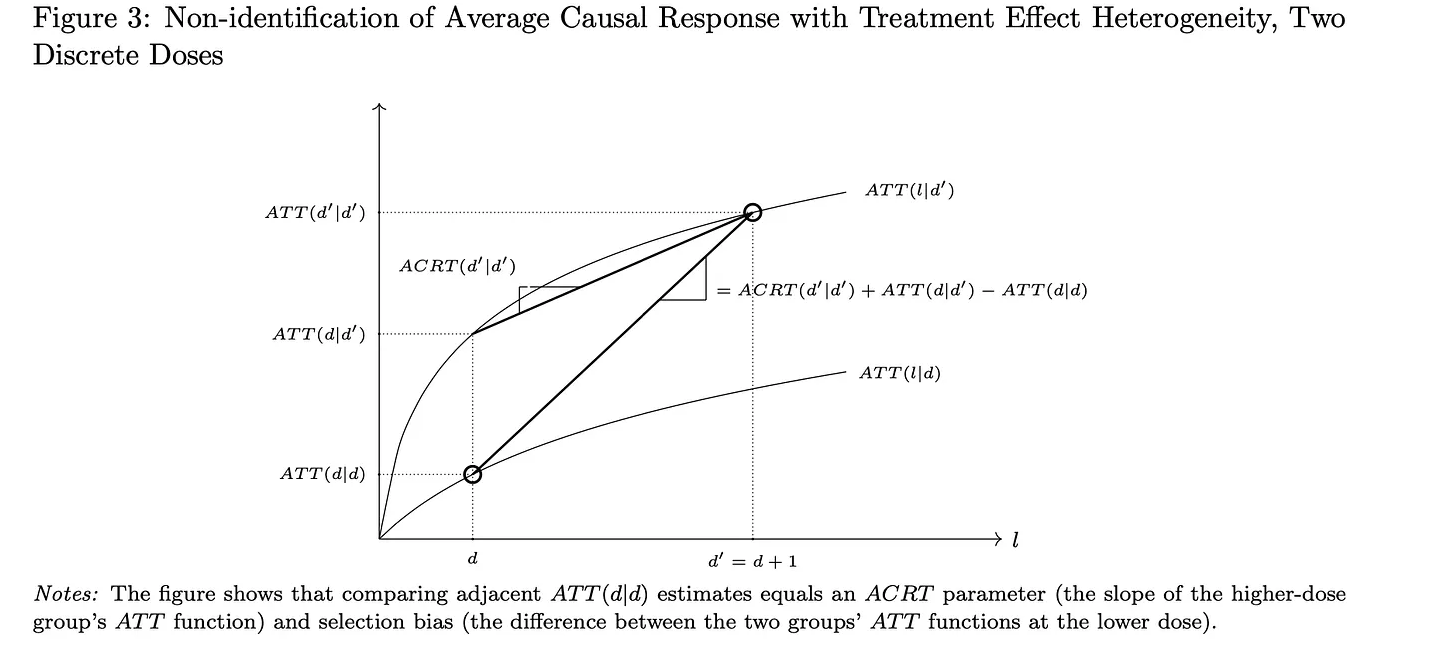
\includegraphics[scale=0.45]{./lecture_includes/continuous5.png}
\end{center}
\end{figure}

\end{frame}

\begin{frame}

\begin{figure}
\begin{center}
             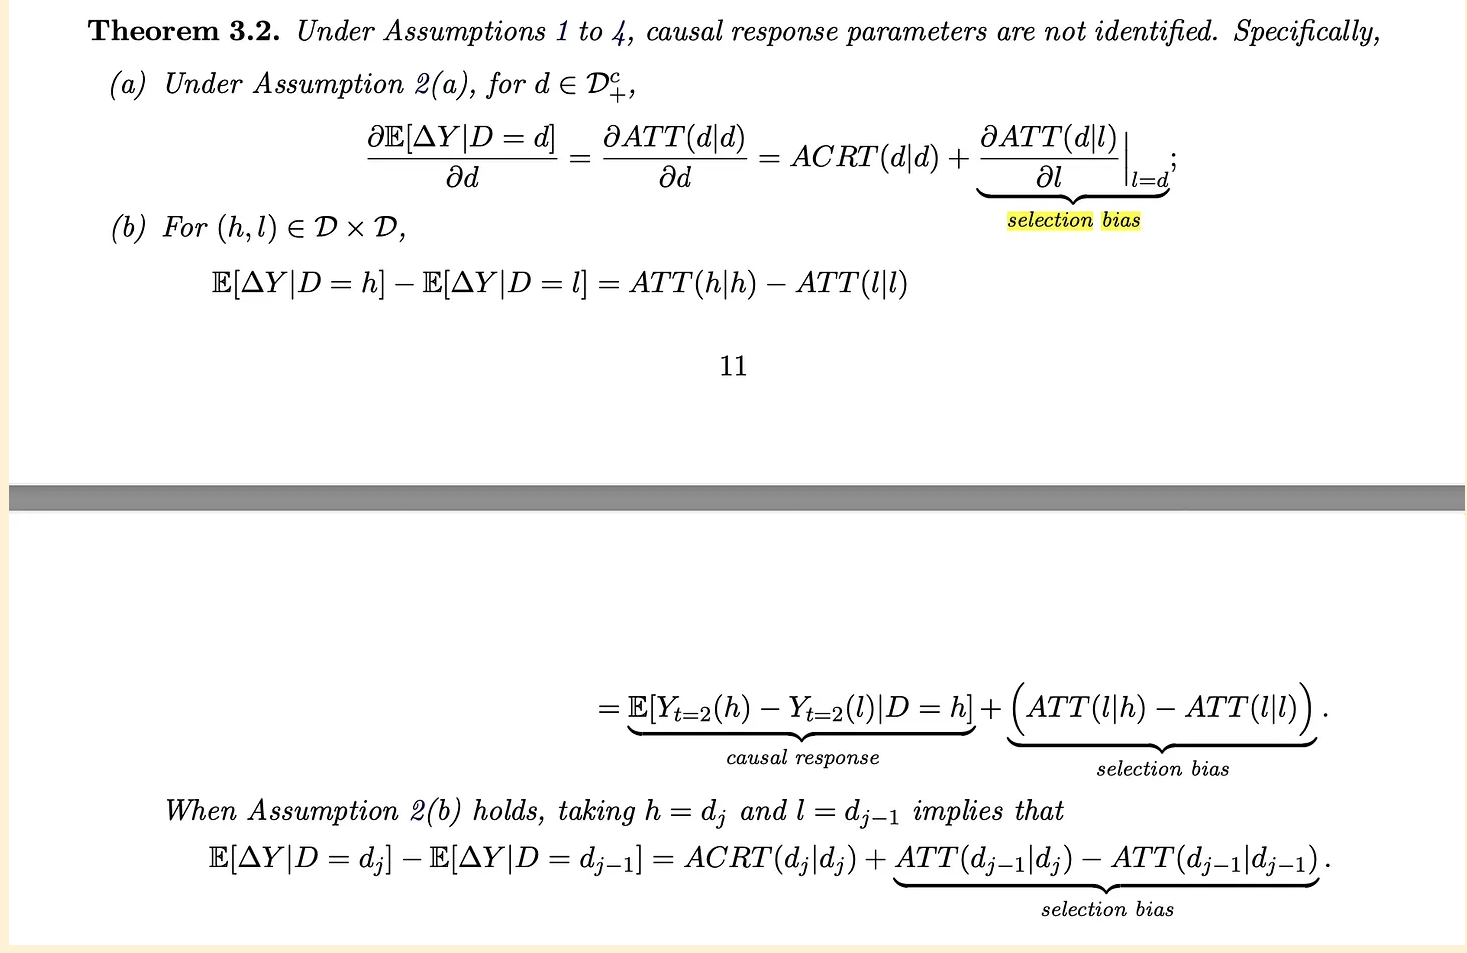
\includegraphics[scale=0.45]{./lecture_includes/continuous6.png}
\end{center}
\end{figure}

\end{frame}

\subsection{Selection bias}


\begin{frame}{Causality and selection bias}

\begin{figure}
\begin{center}
             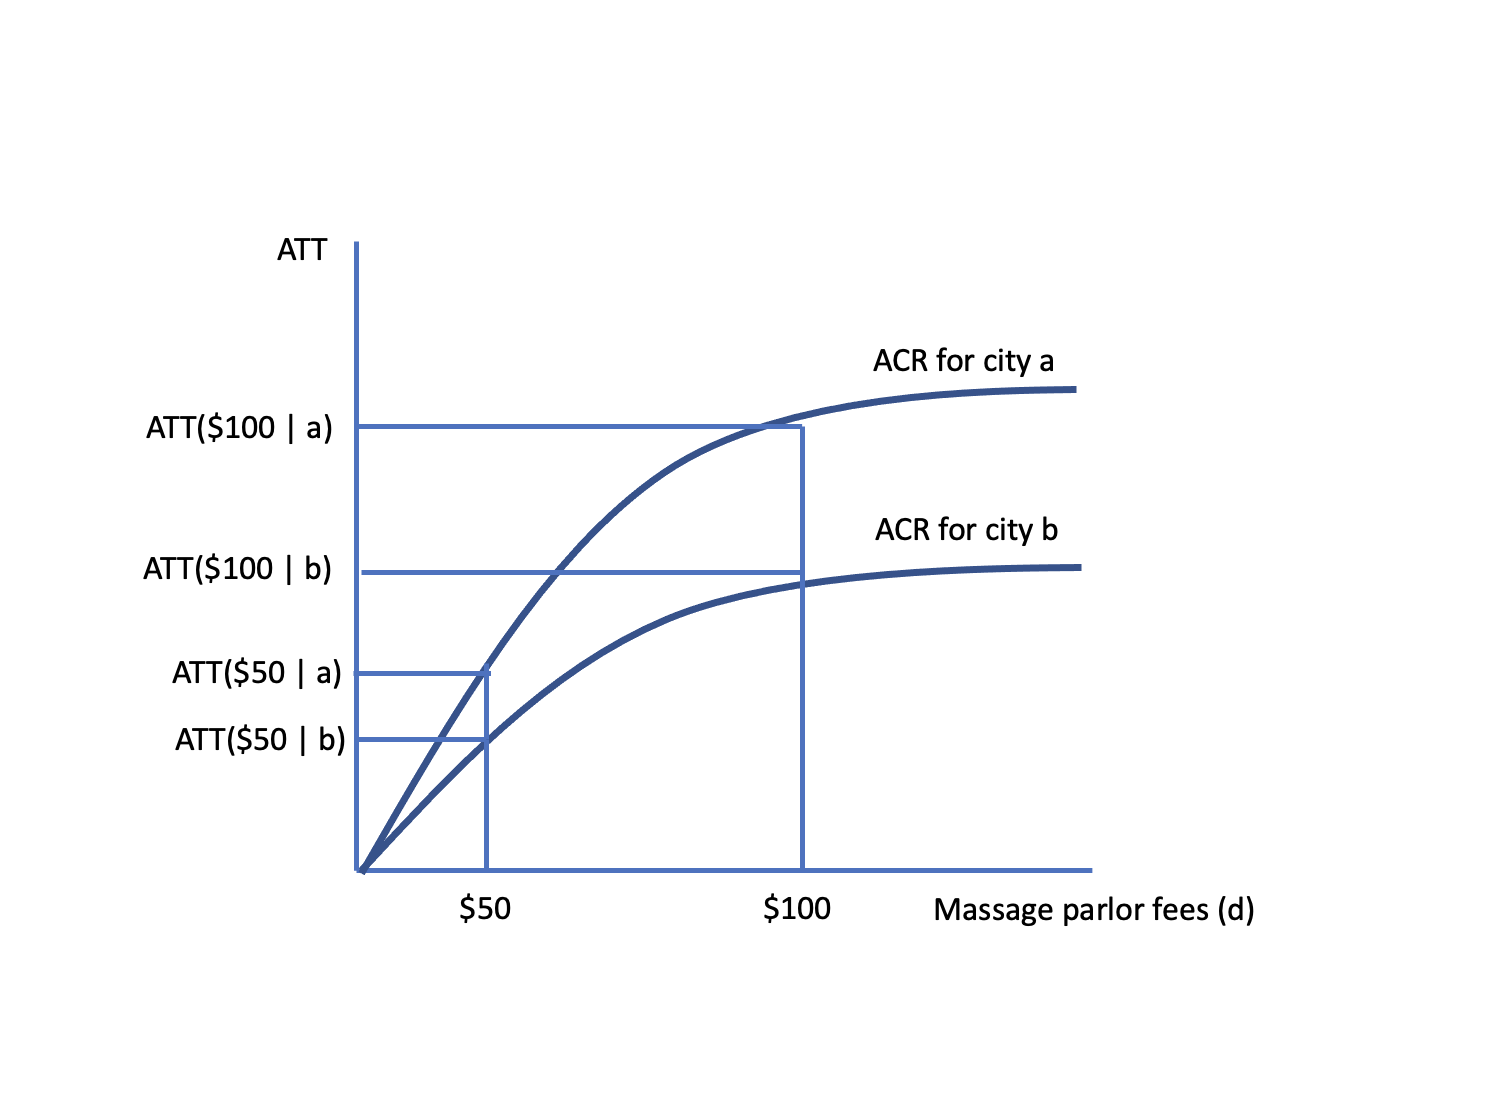
\includegraphics[scale=0.3]{./lecture_includes/acrt_fig2.png}
\end{center}
\end{figure}

Draw the ACRT for top curve and the selection bias from estimation under assumptions 1 to 4.

\end{frame}

\begin{frame}{Interpreting this}

\begin{itemize}
\item Unrestricted heterogenous treatment effects (across dosage levels and across units with difference dose response functions) is not itself the problem
\item If we randomized dosages, then $\textcolor{red}{ATT(d_{j-1} | d_j) - ATT(d_{j-1} | d_{j-1})}=0$
\item Why?  Because then there is no selection on gains from dosages, and average causal response functions are the same for all dosage groups
\item So then when is this a problem?  Sorting on gains
\end{itemize}

\end{frame}

\begin{frame}{Interpreting this}

\begin{itemize}

\item When estimating treatment effects using continuous DiD, you will need to make one of two assumptions
	\begin{enumerate}
	\item Strong parallel trends: Average change in $E[Y^0]$ for the entire sample is the same as the $d$ group
	\item Parallel trends plus homogenous treatment effect functions
	\end{enumerate}
\item Roy model like sorting on gains typically lead to violations of the second condition insofar as there is heterogenous returns to dosages across units
\item So the question you have to ask yourself is do you think that cities are ``optimally setting the minimum wage'' around some given minimum wage?
\end{itemize}

\end{frame}

\begin{frame}{Stronger assumption}

\begin{itemize}

\item I'm really not so sure I think that when it comes to state legislation that I think a Roy model is likely responsible for the equilibrium
\item Solving constrained optimization problems is hard and unlikely is it the case that Florida's ATT and Georgia's ATT are terribly different from one another had both chosen the same minimum wage (but that is the bias)
\item Authors introduce a fifth assumption that will eliminate selection bias, but at the price of restricting heterogeneity

\end{itemize}

\end{frame}



\begin{frame}{Discussion of strong parallel trends}

\begin{quote}
We discuss an alternative but typically stronger assumption, which we call strong parallel trends, that says that the path of outcomes for lower-dose units must reflect how higher-dose units’ outcomes would have changed had they instead experienced the lower dose. Thus, strong parallel trends restricts treatment effect heterogeneity and justifies comparing dose groups. Absent this type of condition, comparisons across dose groups include causal responses but are “contaminated” by an additional term involving possibly different treatment effects of the same dose for different dose groups—we refer to this additional term as selection bias.
\end{quote}

\end{frame}

\begin{frame}{A5: Strong parallel trends}

\begin{figure}
\begin{center}
             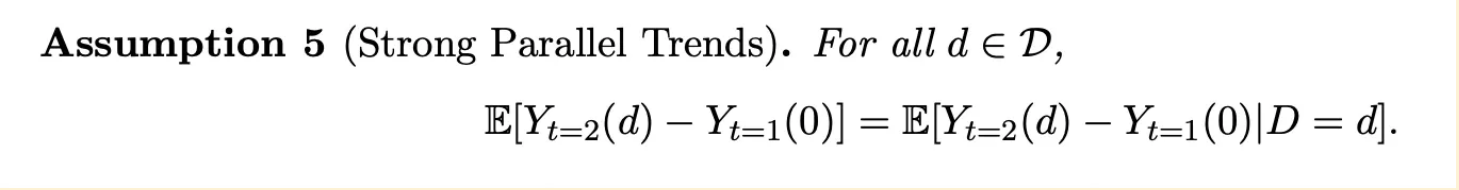
\includegraphics[scale=0.45]{./lecture_includes/continuous7.png}
\end{center}
\end{figure}

\end{frame}


\begin{frame}{Randomization and strong parallel trends}

\begin{itemize}

\item Randomized dosages guarantees that the ACRT are the same across all dosage groups
\item In this situation, strong parallel trends holds because all dosages have the same ATE and ACRT
\item Roy like sorting on dosage may be the biggest challenge you'll face -- schooling stops, family size may not satisfy strong parallel trends

\end{itemize}

\end{frame}






\subsection{Interpreting TWFE}

\begin{frame}{Interpreting TWFE results}

\begin{figure}
\begin{center}
             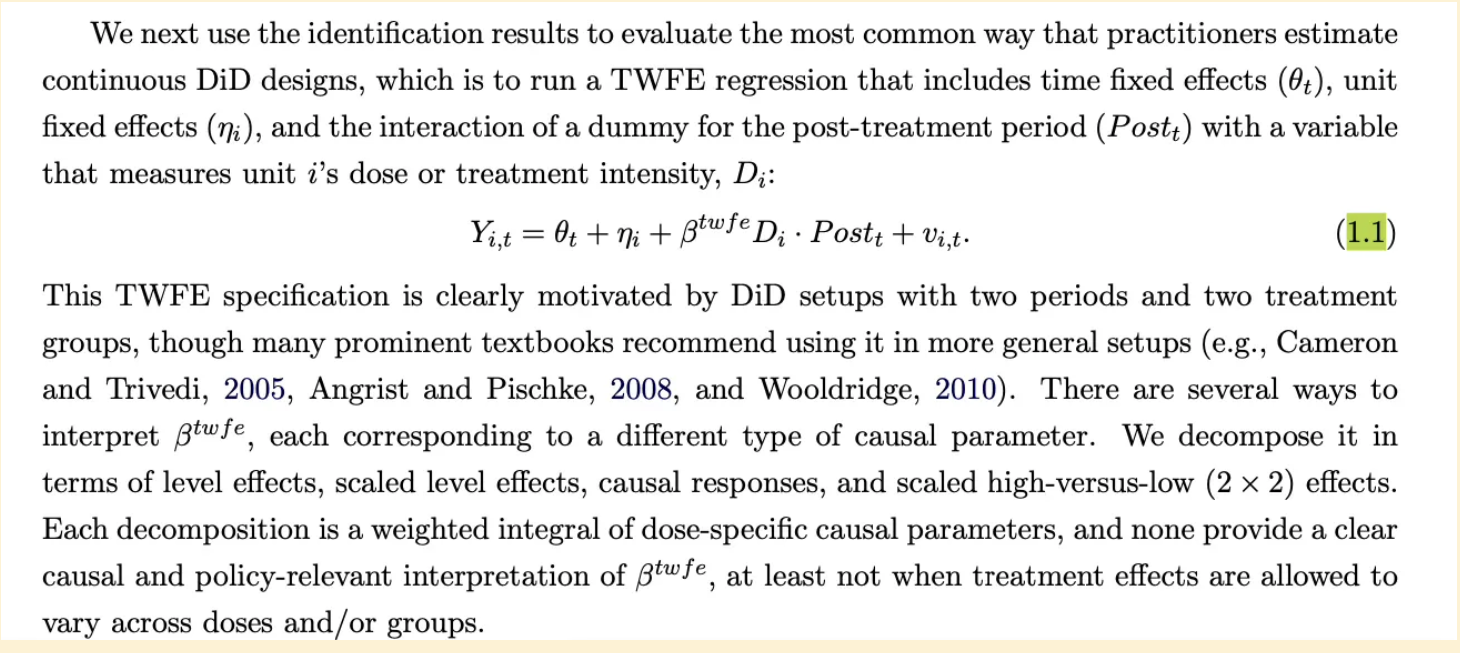
\includegraphics[scale=0.45]{./lecture_includes/continuous8.png}
\end{center}
\end{figure}

\end{frame}


\begin{frame}

\begin{figure}
\begin{center}
             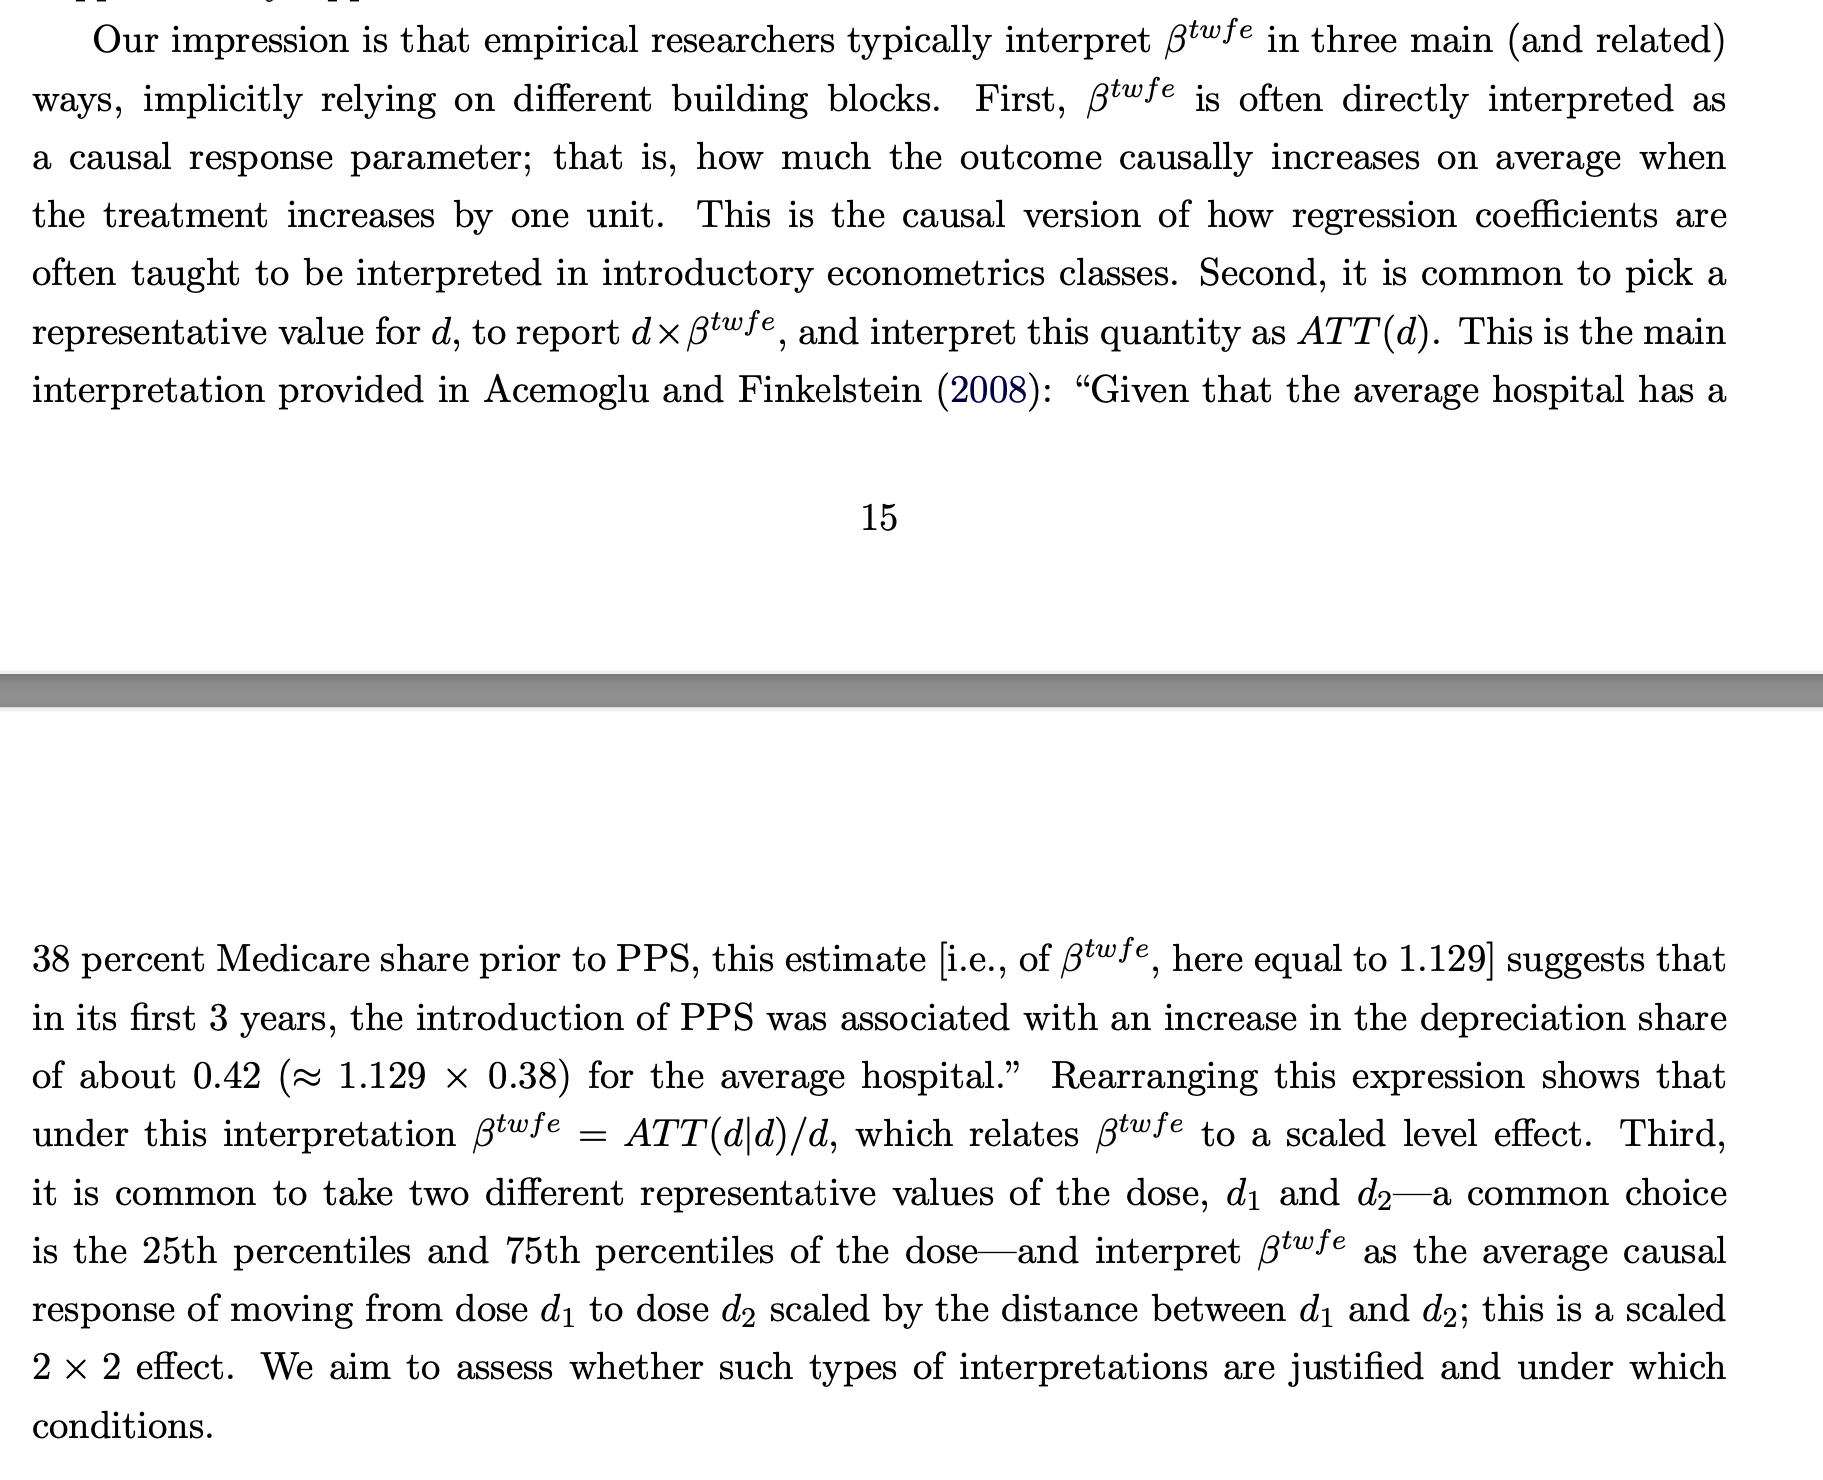
\includegraphics[scale=0.35]{./lecture_includes/continuous12.png}
\end{center}
\end{figure}

\end{frame}





\begin{frame}{Interpreting TWFE}

\begin{figure}
\begin{center}
             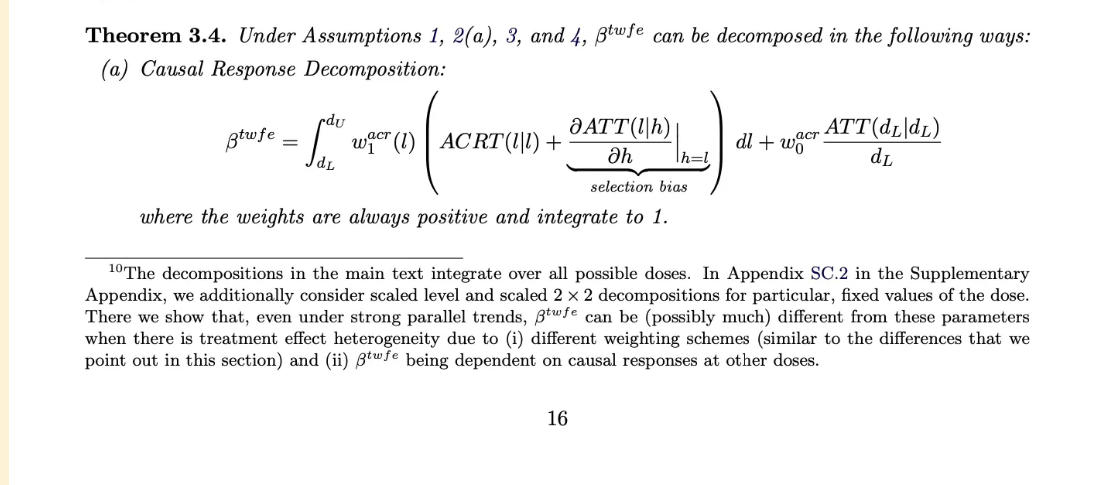
\includegraphics[scale=0.55]{./lecture_includes/continuous9.png}
\end{center}
\end{figure}

\end{frame}


\begin{frame}

\begin{figure}
\begin{center}
             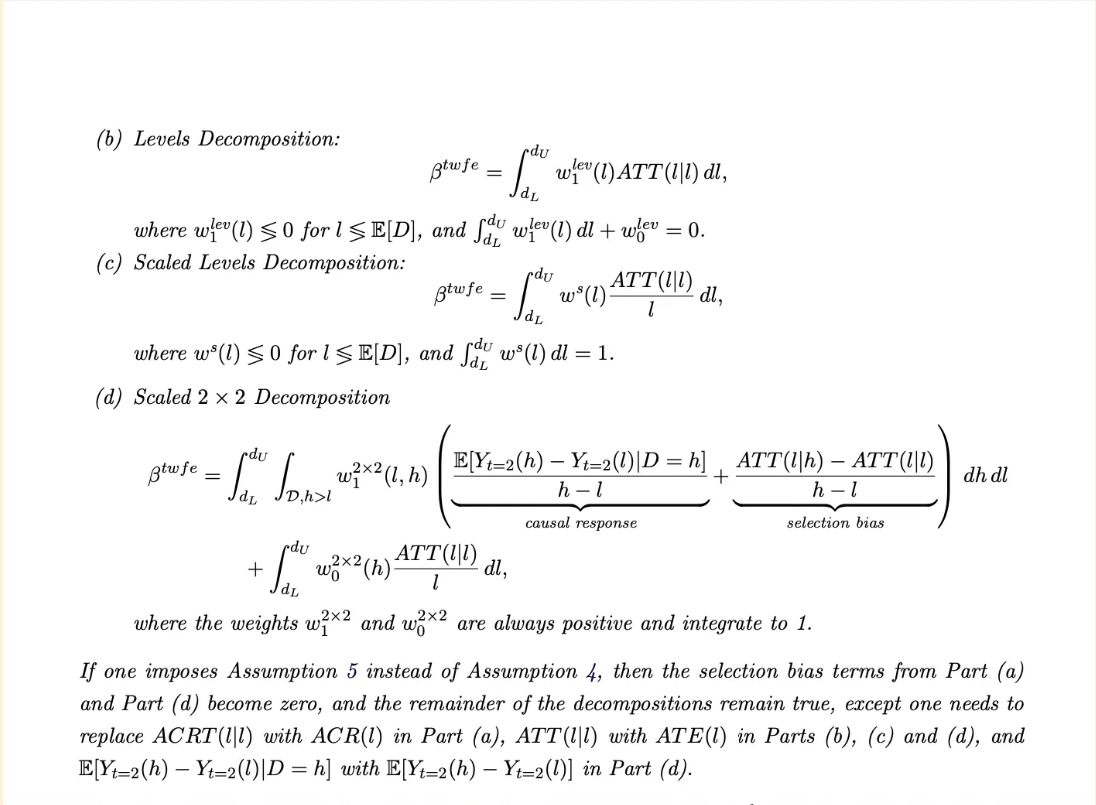
\includegraphics[scale=0.5]{./lecture_includes/continuous10.png}
\end{center}
\end{figure}

\end{frame}
\begin{frame}

\begin{figure}
\begin{center}
             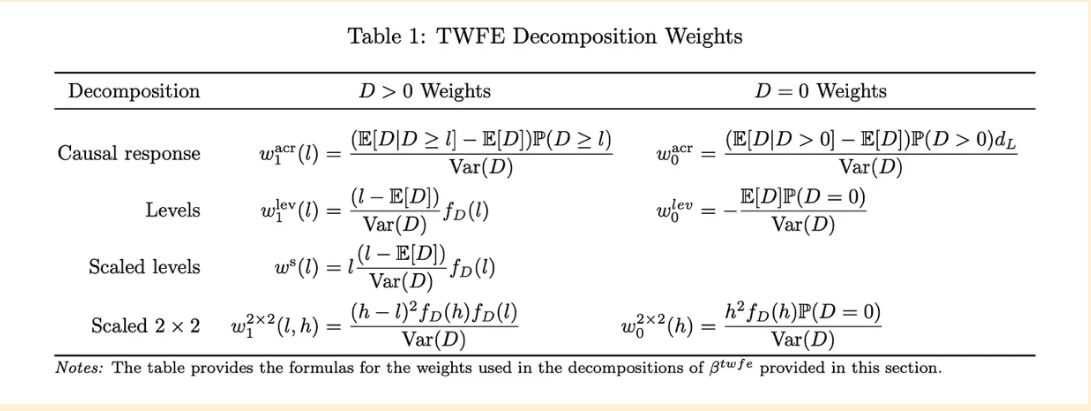
\includegraphics[scale=0.5]{./lecture_includes/continuous11.png}
\end{center}
\end{figure}

\end{frame}








\begin{frame}
\frametitle{Understanding Decomposition Results}

\begin{itemize}
  \item The pattern from decomposition shows distinct impacts of parameter types.
  \item \textbf{Level-effect parameters} (parts b and c):
    \begin{itemize}
      \item $\beta_{twfe}$ is not influenced by selection bias.
      \item Includes negative weights.
    \end{itemize}
  \item \textbf{Comparative doses parameters} (parts a and d):
    \begin{itemize}
      \item $\beta_{twfe}$ carries positive weights.
      \item Encounters selection bias under parallel trends.
    \end{itemize}
\end{itemize}
\end{frame}


\begin{frame}
\frametitle{Addressing Selection Bias and Weighting Schemes}

\begin{itemize}
  \item Parametric linearity restrictions may overlook weighting scheme issues inherent in TWFE regression.
  \item These restrictions do not resolve selection bias problems.
  \item Next, we explore:
    \begin{itemize}
      \item Alternative estimators to TWFE that adjust the weighting scheme.
      \item These alternatives do not rely on the stringent linearity assumption.
      \item Selection bias issues persist and require different solutions.
    \end{itemize}
\end{itemize}
\end{frame}



\begin{frame}{TWFE has many meanings}

\begin{itemize}

\item Today I just wanted to emphasize the basic principles though -- define the parameter, figure out the assumptions, then build the estimators
\item Just running regressions doesn't work once we have heterogenous treatment effects
\item ``Although strong parallel trends removes the selection bias, the weights attached to the causal parameters are still hard to interpret''
\item New papers have developed new methods experimenting with different assumptions, but still waiting on the software
\end{itemize}

\end{frame}




\end{document}






\end{document}



\section{Fuzzy DiD}





\begin{frame}{Sharp DiD}

\begin{itemize}
\item In a ``sharp'' DiD, a group gets treated in period 1, a control group does not
\item Parallel trends allows you to identify ATT
\item We discussed several methods
\item But sometimes the lines between treatment and control groups get ``fuzzy''
\end{itemize}

\end{frame}

\begin{frame}{Fuzziness}

\begin{itemize}
\item In a ``fuzzy'' DiD design, there's growth in treatment occurring among units for reasons other than the treatment assignment in the control group
	\begin{itemize}
	\item They discuss an early 2000s Duflo paper where Indonesia pushed for more primary schooling
	\item Used earlier cohorts as controls bc they were already past the age
	\item But they saw growth in schools too
	\end{itemize}
\item In many applications, the ``treatment rate'' increase more in some groups than in others but there is no group that goes from fully untreated to fully treated
\item But there is no group that also remains fully untreated

\end{itemize}

\end{frame}

\begin{frame}[shrink=10,plain]
\begin{center}
\textbf{Fuzzy estimators}
\end{center}

\begin{itemize}
\item Popular fuzzy estimator (10\% of AERs from 2010-2012) divides DiD of the outcome by the DiD of the treatment 
$$ Wald_{DiD} =  \frac{ 
\bigg (
E[Y_k|Post] - E[Y_k|Pre] \bigg ) - 
\bigg ( E[Y_U|Post] - E[Y_U|Pre] \bigg)
 }
 { \bigg ( 
 E[D_k|Post] - E[D_k|Pre] \bigg) - 
 \bigg ( E[D_U | Post] - E[D_U | Pre] \bigg )} 
$$
\item It's Wald IV in that we scale the reduced form by the first stage but they call it Wald DiD
\item de Chaisemartin and D'Haultfoeuille (2017) estimates the LATE for groups who go from untreated to treated
\end{itemize}

\end{frame}

\begin{frame}{Two proposed estimators}

 Propose two other estimators

	\begin{enumerate}
	\item Time corrected Wald ratio, $Wald_{TC}$ -- relies on PT within subgroup of units sharing the same treatment at the first date
	\item Changes in changes extension, $Wald_{CiC}$ -- extension of Athey and Imbens (2006) ``changes in changes'' paper. Generalizes CiC to fuzzy.  CiC is invariant to outcome scaling but puts restrictions on the full distribution of potential outcomes instead of the mean
	\end{enumerate}
	
\end{frame}

\begin{frame}{Personal takeaway}

\begin{itemize}
\item Two main values of this paper that I found:
	\begin{itemize}
	\item Situations where the control group is getting treated with unrelated policy shocks
	\item Continuous treatments
	\end{itemize}
\item Code to do it is simple but in Stata

\end{itemize}

\end{frame}


\begin{frame}{Most basic notation}

For any random variable, R, we interpret as $R_{dgt}$ as treatment status, treatment group, time \

\bigskip

$R_{101} \sim R | D=1, G=0, T=1$ \

\bigskip

Individual treatment status (D) is whether a unit is treated regardless of group; Group (G) is treatment or control \emph{groups}; Time (T) is before or after \

\bigskip

Sharp: $D = G \times T$; \
Fuzzy: $D\neq G \times T$

\end{frame}

\begin{frame}{Cases under consideration}

Case 1: Share of treated units in control don't change between periods $$E[D_{01}]=E[D_{00}]$$ \\

\bigskip

Wald$_{DiD}$ identifies the LATE parameter for ``switchers'' (i.e., people whose treatment status changed between 0 and 1) if parallel trends hols and if the ATE of treated units at both dates is stable over time; proposes new estimators that don't depend on this \\

\bigskip

Stable ATE isn't required in a typical ``sharp'' DiD

\end{frame}

\begin{frame}{Cases under consideration}

Case 2: Share of treated units changes over time in control $$E[D_{01}]>E[D_{00}]$$\\

\bigskip

Wald$_{DiD}$ identifies the LATE of switchers under PT and stable ATE assumption and LATE of treatment and control group switchers are the same \

\bigskip

Under certain assumptions, their alternative estimator will only be partially identified, and it depends on the size of the change of treated units in the control.  

\end{frame}

\begin{frame}{Fuzzy design assumptions}




\begin{block}{A1: Dominating growth of treated units in the treatment group}
The treatment group is the one experiencing the larger increase in its treatment rate. 
\end{block}
This rules out the case where the two groups experience the same evolution of their treatment rates. Let $R_{gt} \sim R|G=g, T=t$; Assumption 1 implies the following conditions:

\begin{eqnarray*}
E(D_{11})&>&E(D_{10}) \\
E(D_{11}) - E(D_{10}) &>& E(D_{01}) - E(D_{00})
\end{eqnarray*}

\end{frame}


\begin{frame}{Fuzzy design assumptions}

\begin{block}{A2: Stable percent of treated units in the control group}
$0<E(D_{01} ) = E(D_{00})<1$ means there is stable percent of treatment units in the control group.
\end{block}This is a special case where number of treatment units in control group is fixed. 

\end{frame}

\begin{frame}{Fuzzy design assumptions}

\begin{block}{A3: Treatment participation equation}
In the treatment group, no one switches from treatment to control. Formally this is $$D=1\text{ if } V \geq v_{gt}\text{ with every } V \independent T|G$$
\end{block}Where $V$ is the propensity to get treatment, $v_{gt}$ is a threshold specific to each group/time


\end{frame}

\begin{frame}{A little more notation}

\begin{itemize}
\item We say a unit is treated as $D(t) = 1 \{V \geq v_{gt} \}$
\item Switchers are units who go from control to treatment between 0 and 1 $S= \{ D(0) <D(1), G=1 \}$
\item LATE is for switchers: $\Delta=E(Y_{11}(1) - Y_{11}(0) | S$
\item LQTE is also for switchers: $\tau_q = f^{-1}_{y_{11}(1)|S^(q)} - F^{-1}_{y_{11}(0)|S^(q)}$

\end{itemize}

\end{frame}

\begin{frame}{Switcher LATE/LQTE}

Why only switchers?


\begin{itemize}
\item Sometimes only ones affected are switchers; a policy occurs but only eligibility for some.  Switchers end up treated
\item Identifying more than the LATE places more restrictions and this already has like 8 assumptions
\end{itemize}

\end{frame}



\begin{frame}{First estimator: Wald$_{DiD}$}

Commonly used strategy in these fuzzy designs is to normalize the DiD on the outcome by the DiD on the treatment status itself (because remember, in the fuzzy design, units are \emph{becoming} treated as well as \emph{being in treatment groups} \\

\begin{eqnarray*}
Wald_{DiD} = \frac{DiD_Y}{DiD_D}
\end{eqnarray*}

\bigskip



\end{frame}


\begin{frame}{Wald-DiD}

Let $S'= \{ D(0) \neq D(1), G=0 \}$ be control group switchers.  Then we define relevant parameters as:

\begin{eqnarray*}
\Delta ' &=& E(Y_{01}(1) - Y_{01}(0) | S') \\
\alpha &=& \frac{
[P(D_{11}=1) - P(D_{10}=1)]}{DiD_D}
\end{eqnarray*}

\end{frame}

\begin{frame}{Assumptions}

\begin{block}{A4: Parallel trends}
Standard assumption. Not worth repeating for the millionth time.
\end{block}

\end{frame}

\begin{frame}{Assumptions}

\begin{block}{A5: Stable treatment effect over time}
In both groups, the average effect of going from 0 to d units of treatment among units with $D(0)=d$  is stable over time.  This is the same as assuming that among these units, the mean of $Y(d)$ and $Y(0)$ follow the same evolution over time
\end{block}

\begin{eqnarray*}
&&E \bigg [ Y(d) - Y(0) | G, T=1, D(0) = d \bigg ] -\\
&& E \bigg [Y(d) - Y(0) | G, T=0, D(0)=d \bigg ] =0
\end{eqnarray*}for units in the switching population

\end{frame}

\begin{frame}{Assumptions}

\begin{block}{A6: Homogenous treatment effect over time}
Switchers have the same LATE in both groups.  This isn't necessary in sharp DiD, just fuzzy
\end{block}

\end{frame}


\begin{frame}{Wald DiD theorems}

There's a reason we just listed six assumptions.  We need them for this traditional scaled DiD method for fuzzy designs called the Wald DiD.  We'll go in order. 

\begin{block}{Theorem 1: Wald DiD}
If A1, A3-A5 hold, then Wald DiD equals $$\alpha \Delta + (1-\alpha) \Delta '$$but if A2 or A6, then Wald DiD equals $\Delta$
\end{block}


\end{frame}


\begin{frame}{Interpretation of theorem 1: case 1}

Case 1: when treatment grows in the control group, then $\alpha>1$.  Then if we assume A1, A3-A5, a lot of things cancel out under A1, A3-A5, but the Wald DiD becomes a weighted \emph{difference} of the LATEs of treatment and control group switchers in period 1. \\

\bigskip

Since it is a difference in LATEs, then even two positive LATEs can flip sign if the first is less than the second. \\

\bigskip 

But if you assume A6, you just get the LATE.  

\end{frame}

\begin{frame}{Interpreting theorem 1: case 2}

Case 2: When treatment diminishes in controls, then $\alpha<1$. \\

\bigskip

Then under A1, A3-A5, Wald DiD will equal a weighted average of LATEs of treatment and control group switchers in period 1. \\

\bigskip

This quantity will not reverse signs, but won't equal the LATE without A6.

\end{frame}

\begin{frame}{Interpreting theorem 1: case 3}

Case 3: Treatment rate is stable in control, then $\alpha=1$ and Wald DiD will equal LATE under A1, A3-A5. \\

\bigskip

This requires that the ATE among units treated at T=0 remain stable over time -- necessary condition. \\

\bigskip

Under A1, A3-A4, Wald DiD is equal to LATE plus a bias term involving several LATEs, and unless they cancel out exactly, Wald DiD will be different from the LATE

\end{frame}

\begin{frame}{Alternative estimators}

\begin{itemize}
\item Wald TC -- Time Corrected Wald DiD
\item Wald CiC -- Changes in changes generalization to fuzzy design
\end{itemize}

Now we review alternative assumptions under which Wald TC or Wald CiC identify the LATE of switchers in the fuzzy.  First let's look at Wald TC which won't depend on A4-A5.

\end{frame}

\begin{frame}{Alternative assumptions for the Wald TC}

\begin{block}{A4': Conditional parallel trends}
This requires $Y(0)$ mean average follow the same trends as all the other groups.
\end{block}

\end{frame}

\begin{frame}{Wald TC estimator}

Wald TC equals $$\frac{
E(Y_{11}) - E(Y_{10} + \delta_{D_{10}})}{E(D_{11} - E(D_{10}}$$where $$\delta_d = E[Y_{d_{01}}] - E[Y_{d_{00}}]$$ which is the change in mean outcome between periods 0 and 1 for controls and treatment status $d$ (not groups T and C -- individual units $d$). 

\end{frame}


\begin{frame}{Theorem 2}

\begin{block}{Theorem 2 and the Wald TC}
If A1-A3 and A4', then Wald TC equals $\Delta$
\end{block}

Note that: Wald TC equals

$$
\frac{
E  (Y | G=1,T=1) - 
E(Y+ (1-D)\delta_0 + D \delta_1 | G=1, T=0 )}{
E(D|G=1,T=1) - E(D|G=1,T=0)}$$

This is almost the Wald DiD ratio except for that second term with the $Y+(1-D)\delta_0 + D\delta_1$ instead of just $Y$. \\

\bigskip 

This arises because time can independently affect the outcome.  \\

\bigskip

When treatment is stable for a group $G$, then $\delta_0=0$. \\


\end{frame}


\begin{frame}{Comment on Theorem 2}

Wald TC equals

$$
\frac{
E  (Y | G=1,T=1) - 
E(Y+ (1-D)\delta_0 + D \delta_1 | G=1, T=0 )}{
E(D|G=1,T=1) - E(D|G=1,T=0)}$$

The numerator of Wald TC compares the mean outcome in the treatment group in the post period 1 to the counterfactual mean we would have had if switchers had remained untreated.  \\

\bigskip 

Then normalized by the change in switching, we get the LATE for switchers

\end{frame}

\begin{frame}{Wald CiC}

Here we have continuous outcomes and an estimator for quantiles of the LATE called LQTE.  New assumption is complicated but is needed for the Wald CiC

\end{frame}

\begin{frame}{Assumptions for changes in changes Wald ratio}


\begin{block}{A7: Monotonicity and time invariance of unobservables}
Potential outcomes are strictly increasing functions of some scalar unobserved heterogeneity term whose distribution is stationary over time.  Also imposes the distribution of that unobserved heterogeneity be stationary within subgroups of units sharing the same treatment status at baseline.
\end{block}

\end{frame}

\begin{frame}{Data restrictions}

\begin{block}{A8: Data restrictions}
First, Y must have the same support in each of the eight $D \times G \times T$ cells (common support).  Second, the distribution of Y be continuous with positive density in each of the eight cells.
\end{block}

This will allow us to bound treatment effects (Athey and Imbens 2006). Now the ugliest estimator ever.

\end{frame}

\begin{frame}{Wald CiC estimator}

Let $Q(y) = F_{Y_{01}}^{-1} \cdot F_{Y_{00}}(Y)$ be the quantile-quantile transform of $Y$ from period 0 to 1 in the control group.  Also let:

\begin{eqnarray*}
F_{CiC,d(Y)} = \frac{
P(D_{11}=d) F_{Y_{d11}} - 
P(D_{10}=d) F_{Y_{d10}}}{
P(D_{11}=d) - P(D_{10}=d)}
\end{eqnarray*}And our Wald CiC estimator is:

\begin{eqnarray*}
W_{CiC} = \frac{
E(Y_{11}) - E(Q_{D10}(Y_{10})}
{E(D_{11}) - E(D_{10})}
\end{eqnarray*}

\end{frame}

\begin{frame}{Theorem 3: Wald CIC}

\begin{block}{Theorem 3: Wald CiC}
Under A1-A3 and A7-A8, then $W_{CiC}$ is the LATE and equivalently we get the LQTE
\end{block}

\footnotesize
\begin{eqnarray*}
W_{CiC} = \frac{
E(Y|G=1,T=1) - 
E((1-D)Q_0(Y) + DQ_1(Y) | G=1, T=0}{
E(D|G=1,T=1) - E(D|G=1,T=0)}
\end{eqnarray*}

\end{frame}

\begin{frame}{Comment on theorem 3}

Almost the standard Wald DiD except for that $(1-D)Q_0(Y) + DQ_1(Y)$ instead of Y in the second term of the numerator.  So again, we are simply making adjustments for the fuzziness but under different set of assumptions. This term accounts for the fact that time directly affects the outcome, but in a CiC setup.

\end{frame}

\begin{frame}{Which to use}

It's about choosing your poison.  Do you want A4' or A7? 

\bigskip

When T and C have different outcome distributions conditional on D in the first period, then scaling of the outcome may have large effect on the Wald-TC.  Whereas Wald-CiC isn't sensitive to the scaling of Y.

\bigskip

But when the two groups have similar outcome distributions conditional on D in the first period, Wald-TC may be preferable as A4' only restricts the mean of the potential outcomes, whereas Wald-CiC restricts the entire distribution

\end{frame}

\begin{frame}{Extensions to non-binary, ordered treatment}

\begin{block}{Theorem 6}
Under continuous treatments, the estimators we've been considering are equal to the average causal response parameter that Angrist and Imbens (1995) discuss.  This parameter is a weighted average over all values of $d$ of the effect of increasing treatment from $d-1$ to $d$ for any switchers where treatment status goes from strictly below to strictly above $d$ over time.
\end{block}

Theorem 6 extends to a continuous treatment.  Under theorem 6, each of the estimators is identifying a weighted average of the derivative of potential outcomes with respect to changing $d$

\end{frame}

\begin{frame}{Stata code}

Only code I know of at the moment is the fuzzydid the authors published in Stata Journal.  But it allows you to specify which estimator.  Here's sample code for Wald DiD:

\bigskip

\texttt{fuzzydid lngonf g_decr post1 inverse_fee, did breps (1000) cluster(county1)}

where $g_decr$ is the treatment group dummy, post1 is the post period dummy, and $inverse_fee$ is our continuous treatment variable. We specify the Wald DiD by noting did after the comma.

\end{frame}

\begin{frame}{Concluding remarks}

\begin{itemize}
\item Paper is hard but worth it.  It's possible your controls are getting treated for unrelated reasons, but this is testable
\item The Wald DiD is a conventional approach but suffers bias without a layering in of assumptions
\item Alternative estimators for when control group stabilization isn't possible or you don't want to impose treatment effect homogeneity are available
\item fuzzydid can handle continuous treatments as well as dummies.
\end{itemize}

\end{frame}



